\documentclass[11pt,a4paper]{article}

% Generated by paper/sync_main_tex.mjs from manuscript_print.html; edit build_publication_pdf.mjs and re-run both scripts,
% or edit this file and make the same change in build_publication_pdf.mjs.
\usepackage[utf8]{inputenc}
\usepackage[T1]{fontenc}
\usepackage{geometry}
\geometry{margin=1in}
\usepackage{amsmath,amssymb,amsfonts,amsthm}
\usepackage{booktabs}
\usepackage{array}
\usepackage{graphicx}
\usepackage{hyperref}
\usepackage{xcolor}
\usepackage{enumitem}
\usepackage{caption}
\usepackage{algorithm}
\usepackage[noend]{algpseudocode}
\usepackage{natbib}
\usepackage{setspace}
\onehalfspacing

\hypersetup{
    colorlinks=true,
    linkcolor=blue!70!black,
    citecolor=blue!70!black,
    urlcolor=blue!70!black
}

\theoremstyle{definition}
\newtheorem{proposition}{Proposition}
\newtheorem{invariant}{Governance Invariant}

\title{\textbf{Governing Human--AI Collaborative Project Workflows in Multi-Platform Digital Delivery: A Design Science Study of Auditable Handoffs and Idempotent Release Operations}}

\author{
  \textbf{HuaiCheng Sheng}$^{1,*}$ \\
  \small $^{1}$Agentic Work Lab, Hangzhou Chengxin Holding Group Co., Ltd., Hangzhou, Zhejiang, China \\
  \small $^{*}$Corresponding author. E-mail: \texttt{ZackSheng@gmail.com} \,|\, ORCID: \href{https://orcid.org/0009-0003-2900-6377}{\texttt{0009-0003-2900-6377}}
}

\date{November 2026}

\begin{document}

\maketitle

\begin{abstract}
\noindent
\textbf{Context:} When large language model (LLM) agents move from conversation to execution, project governance must control actions on external platforms that cannot be undone. An uncertain submission that is retried can be published twice, and descriptive metrics are easily reported as evidence of AI-driven gains. \\
\textbf{Objective:} Following Design Science Research (DSR) and stage-gate project control theory, we design and evaluate a human-in-the-loop (HITL) governance framework for multi-agent, multi-platform digital delivery, implemented in two open-source artifacts, \emph{Agentic Work Lab} and \emph{PublishOps CrossCast}. \\
\textbf{Method:} The framework has four layers: (1) a deterministic owner, stop-flag and due-time gate (\texttt{planRun}); (2) binding of each release command to the SHA-256 digest of the reviewed plan, with SHA-256 media checks; (3) a receipt state machine that records an \texttt{UNKNOWN} state before the single final submission and never re-submits automatically; and (4) independent read-back with escalation to a person. We evaluate it in a nine-day field deployment (26 October--3 November 2026) in one creator--engineering laboratory, using a 69-record operational journal, a scheduled heartbeat trace, a five-platform release of one film, 2,737 offline test functions, 30 SHA-256-recorded video versions (2.21 GB) and a 55-record channel snapshot. \\
\textbf{Results:} The journal records one platform write and no replayed upload. The heartbeat started 24.992 s late and ran 31.175 s without task errors. When Douyin's read-back timed out, the receipt stayed \texttt{UNKNOWN}, nothing was re-submitted, and the owner confirmed the work by phone. In one instrumented Instagram run, 380.551 s of the 412.217 s publish command (92.32\%) was the wait after the single Share, spanning transfer, processing and confirmation. \\
\textbf{Conclusions:} Here, agentic delivery was governed by deterministic gates, content-bound approvals and at-most-once submission with human reconciliation rather than by prompt instructions. The evidence is single-case and descriptive; code, data and a script that recomputes every reported figure are public.

\vspace{0.5em}
\noindent
\textbf{Keywords:} Project Management Governance; Human--AI Collaboration; Multi-Agent Workflows; Design Science Research; Idempotent Release Engineering; Stage-Gate Control; PublishOps
\end{abstract}

\newpage
\section*{Highlights}
\begin{itemize}[leftmargin=1.5em]
    \item A four-layer stage-gate design governs human--AI delivery to five platforms
    \item Receipts are saved as UNKNOWN before the one final submit; no auto re-submit
    \item A 69-record field journal shows one platform write and no replayed upload
    \item In one Instagram run, 92.32\% of the publish command was the wait after Share
    \item Descriptive channel data are kept apart from causal claims about AI output
\end{itemize}

\newpage

\section{Introduction}
\label{sec:1}

The rapid maturation of Large Language Models (LLMs) and tool-using agents is changing how projects in software engineering and digital operations are run \citep{Holzmann2022, Muller2024, Wang2024Agent}. Unlike automation scripts that execute fixed subroutines within narrow integration boundaries, agentic workflows deploy heterogeneous foundation models---reasoning-oriented coding agents, interface construction agents and scheduled monitoring agents---to collaborate on multi-stage deliverables \citep{Wu2023AutoGen, Hong2023MetaGPT, Qian2024ChatDev}. In digital media production, release engineering and outreach operations, such multi-agent arrangements promise less manual coordination and shorter turnaround \citep{Raisch2021, Berente2021}.

Deploying autonomous or semi-autonomous agents into production, however, exposes governance problems that classical project management methods \citep{PMI2021, Kerzner2022} and conversational multi-agent frameworks were not designed to address. Four failure modes can arise when LLM agents act on shared repositories and external platforms:

\begin{enumerate}[leftmargin=1.8em]
    \item \textbf{Multi-Agent Handoff Drift and Role Ambiguity:} When several specialized models (here, GPT/Codex for scripts, code-driven video and backend verification; Claude for interface construction; and DeepSeek for scheduled monitoring) work asynchronously on shared project state, context boundaries can degrade. Without ownership locks and explicit acceptance gates, an agent woken by a schedule may repeat a task another instance has claimed, overwrite approved revisions or act on a stale checklist \citep{Whyte2016, Qian2024ChatDev}.
    \item \textbf{Non-Idempotent External Side Effects under Platform Uncertainty:} Release operations across Bilibili, YouTube, X, Douyin and Instagram mix official APIs with stateful browser sessions. Network interruptions, transcoding queues, verification challenges or read-back timeouts can leave a submission in an indeterminate (\texttt{UNKNOWN}) state \citep{Schneider1990, Kleppmann2017}. Unlike payment and cloud APIs, these web submission flows offer no idempotency key that would let the platform discard a duplicate \citep{Helland2012}, so a retry loop that reads a missing confirmation as failure may publish twice, disturb playlist order or trigger rate limits.
    \item \textbf{Opaque Quality Degradation in Generative Deliverables:} One-shot generative pipelines can introduce localized defects---single-frame flashes before transitions, audio--video drift, clipped audio or mobile overlay cropping---that pass superficial completion checks. Without editable intermediate representations and signal-level checks, repairing one defect means regenerating the whole deliverable and discarding validated segments.
    \item \textbf{Epistemic Confounding in Project Performance Evaluation:} AI adoption is often reported with claims of labour savings or audience growth that the underlying data cannot support \citep{Raisch2021}. Comparing historical human-led output with a newly launched AI-assisted series confounds exposure age (years of cumulative traffic versus days), topic and platform recommendation dynamics, and counting generated drafts as delivered work hides the human review and rework that acceptance required.
\end{enumerate}

To address these problems, this study adopts Design Science Research (DSR) \citep{Hevner2004, Peffers2007, Gregor2013, Venable2016} to build and evaluate a human-in-the-loop (HITL) governance framework and release operations system: \textbf{Agentic Work Lab} and its standalone multi-platform release engine \textbf{PublishOps CrossCast} (\texttt{vpub}). Rather than treating AI governance as prompt engineering, we formulate multi-agent delivery as a verifiable stage-gate control system \citep{Cooper1990, Conforto2016, Bianchi2022} backed by content digests, frame-level quality checks and fault-tolerant state transitions.

Specifically, this paper investigates three research questions (RQs):

\begin{itemize}[leftmargin=1.8em]
    \item \textbf{RQ1 (Governance Architecture \& Handoff Control):} How can stage-gate project management principles be formalized into deterministic software invariants to govern multi-model handoffs (GPT/Codex, Claude and DeepSeek) and prevent unauthorized or duplicate autonomous actions?
    \item \textbf{RQ2 (Idempotent Release Engineering \& Fault Recovery):} How can a persistent receipt state machine coordinate multi-platform releases, in-place revisions and authorized deletions across API and browser-automated channels when post-submission verification meets timeouts or human authentication barriers?
    \item \textbf{RQ3 (Empirical Latency, Quality \& Epistemic Validation):} What operational characteristics, latency bottlenecks, defect-repair patterns and methodological boundaries are observed when this architecture is used in a nine-day field deployment across five platforms?
\end{itemize}

The contributions are fivefold:

\begin{enumerate}[leftmargin=1.8em]
    \item \textbf{A Four-Layer Agentic Project Governance Framework:} We synthesize stage-gate control \citep{Cooper1990}, configuration management \citep{Whyte2016} and human-centered automation \citep{Parasuraman2000, Shneiderman2020} with commit-protocol reasoning from distributed systems (Section 2.4) into four enforceable layers: (i) a sole-operator and temporal scheduling gate, (ii) plan-hash and media-integrity binding, (iii) an idempotent receipt state machine with \texttt{UNKNOWN}-state suppression, and (iv) independent read-back, in-place revision and HITL handoff.
    \item \textbf{Algorithms with Stated Assumptions:} Three algorithms govern job planning (Algorithm 1), publication with a receipt persisted before the final submission (Algorithm 2), and identity-bound revision and consent-bound deletion (Algorithm 3); Proposition 1 states the conditions under which automated re-submission cannot occur.
    \item \textbf{Open-Source Reference Implementation:} We describe the architecture and evolution of \emph{PublishOps CrossCast} from \texttt{v0.2.2} to commit \texttt{75b7abc} (PR \#30), whose test suite grew from 2,009 to 2,737 test functions between the \texttt{v0.16.0} release and that commit, together with dependency-free Node.js verification scripts in \emph{Agentic Work Lab}.
    \item \textbf{Field Evidence and a Latency Profile:} We report the system's behaviour in a 69-record operational journal, 30 SHA-256-recorded video versions (2.21 GB), a 13,034-frame defect scan, a crash-recovery check on a private upload, and a five-platform release in which one in-doubt submission was held without re-submission. In one Instagram publication, the wait after Share accounted for 92.32\% of the publish command, which motivates persisting submission state before that wait.
    \item \textbf{A Protocol for Auditable AI Project Reporting:} We demonstrate reporting rules that keep observational receipts apart from causal inference, guarding against exposure-age confounding when human-led ($n$ = 45) and AI-assisted ($n$ = 10) cohorts are compared.
\end{enumerate}

The study is a single-case design science evaluation: its claims concern how the mechanisms behaved and why, not how often such failures occur across projects (Section 7.4).

\section{Related Work and Theoretical Background}
\label{sec:2}

\subsection{Project Management Governance and Stage-Gate Control in the AI Era}
\label{sec:2.1}

Classical project management emphasizes structured control mechanisms---Work Breakdown Structures, configuration management and Stage-Gate reviews---to manage technical uncertainty and enforce accountability across project phases \citep{Cooper1990, Whyte2016, PMI2021, Kerzner2022}. In Cooper's Stage-Gate model and in hybrid agile--stage-gate frameworks \citep{Conforto2016, Bianchi2022}, iterative work within a stage is separated from downstream commitment by decision gates, each with predefined deliverables, explicit criteria and a gatekeeper who decides whether to proceed, recycle, hold or stop. Project governance research separates the framework that assigns decision rights and accountability from the management of execution itself \citep{Too2014}; in delivery terms, governance decides who may authorize an irreversible step, and on what evidence.

Recent scholarship examines how artificial intelligence changes project governance, decision authority and human--machine agency \citep{Holzmann2022, Muller2024}. \citet{Raisch2021} describe the tension between automation and augmentation in management: removing human judgment from critical loops invites drift and brittle failure under novel cases, whereas isolated augmentation fails to scale. Work on human--automation interaction argues that reliable socio-technical systems combine high automation with high human control through transparent audit trails, explicit pre-authorization and graceful exception handoffs \citep{Parasuraman2000, Amershi2019, Shneiderman2020}. Much of the project management literature on AI, however, relies on conceptual typologies or expert Delphi surveys \citep{Holzmann2022}; translating stage-gate governance into software-enforced invariants for live, multi-model agents remains largely unaddressed.

\subsection{Multi-Agent LLM Workflows and Coordination Vulnerabilities}
\label{sec:2.2}

Reasoning-and-acting paradigms such as ReAct \citep{Yao2023ReAct} and Reflexion \citep{Shinn2023Reflexion} have led to multi-agent frameworks including AutoGen \citep{Wu2023AutoGen}, MetaGPT \citep{Hong2023MetaGPT} and ChatDev \citep{Qian2024ChatDev}. MetaGPT encodes Standardized Operating Procedures into role-specific prompts (product manager, architect, engineer, QA), while ChatDev structures software development as a sequential chat chain. These frameworks perform well on self-contained coding benchmarks \citep{Wang2024Agent}, but continuous multi-platform operations expose three gaps:

\begin{itemize}[leftmargin=1.8em]
    \item \textbf{No Cross-Process Execution Locks:} Prompt-based procedures do not prevent two agent sessions (for example, an interactive coding session and a scheduled heartbeat) from mutating the same browser profile or checklist at once.
    \item \textbf{No Binding of Approval to Artifact Content:} In conversational handoffs, an agent may approve a text summary while the binary artifact on disk is an older, unpatched version or has been misread.
    \item \textbf{Unbounded Retries on External Timeouts:} Tool-calling loops commonly treat timeouts or selector failures as transient errors and invoke the tool again, which duplicates a publication whenever the platform had in fact accepted the first submission.
\end{itemize}

\subsection{DevOps, Release Engineering, and Idempotent State Machines}
\label{sec:2.3}

In software engineering, Continuous Integration and Continuous Delivery (CI/CD) pipelines reduce deployment risk through automated build verification, immutable artifact digests and staged rollouts \citep{Humble2010, Bass2015, Adams2016, Shahin2017, Leite2019}. A cornerstone of fault-tolerant distributed systems and transaction processing is \emph{idempotency}: repeating an operation, or recovering from an interrupted request, must not produce duplicate side effects \citep{Schneider1990, gray1992transaction, Kleppmann2017}. Payment and cloud APIs commonly accept a client-chosen idempotency key so that the server can discard duplicates \citep{Helland2012}; browser-driven submission to consumer platforms offers no such key, so the client alone must decide whether a second attempt is safe. Table 1 contrasts multi-agent frameworks, CI/CD pipelines and generic upload scripts with the proposed \emph{Agentic Work Lab} and \emph{PublishOps CrossCast} architecture across eight governance dimensions.

\begin{table}[htbp]
\centering
\caption{Comparative analysis of multi-agent frameworks, release pipelines and the proposed governance architecture across eight governance dimensions. Entries describe built-in mechanisms as documented; ``No'' means not provided as a built-in mechanism, not that it cannot be built on top. Upload helpers are characterized generically.}
\label{tab:1}
\scriptsize
\setlength{\tabcolsep}{3pt}
\begin{tabular}{>{\raggedright\arraybackslash}p{0.170\textwidth}>{\raggedright\arraybackslash}p{0.098\textwidth}>{\raggedright\arraybackslash}p{0.098\textwidth}>{\raggedright\arraybackslash}p{0.098\textwidth}>{\raggedright\arraybackslash}p{0.098\textwidth}>{\raggedright\arraybackslash}p{0.107\textwidth}>{\raggedright\arraybackslash}p{0.107\textwidth}>{\raggedright\arraybackslash}p{0.116\textwidth}}
\toprule
\textbf{Framework / System} & \textbf{Multi-Model Handoffs} & \textbf{Temporal \& Owner Gate} & \textbf{Crypto Plan \& SHA-256 Lock} & \textbf{Hybrid API + Pipe Browser} & \textbf{\texttt{UNKNOWN} Latch (Zero Retry)} & \textbf{Identity-Bound Edit/Delete} & \textbf{Epistemic \& Non-Causal Audit} \\
\midrule
\textbf{AutoGen} \citep{Wu2023AutoGen} & Conversational chat loops & No native lock & No & External tools only & No (standard retry) & No & No \\
\textbf{MetaGPT} \citep{Hong2023MetaGPT} & Prompt-level SOP roles & Sequential memory & No & No & No & No & No \\
\textbf{ChatDev} \citep{Qian2024ChatDev} & Dual-agent chat chain & Phase-level only & Git commit only & No & No & No & No \\
\textbf{Standard CI/CD} \citep{Humble2010} & Static pipeline stages & Runner queue locks & Artifact SHA-256 & REST APIs only & API-dependent & Rollback scripts & Build logs only \\
\textbf{Open-Source Upload Helpers} (generic) & Single-script execution & Cron timer only & No plan-hash lock & Browser form fill & No (risks double post) & No read-back verification & No \\
\midrule
\textbf{\textbf{Agentic Work Lab \& CrossCast (Ours)}} & \textbf{File-mediated state handoffs (GPT/Claude/DS)} & \textbf{Deterministic \texttt{planRun} + OS lock} & \textbf{\texttt{-{}-confirm} Plan Hash + Stream SHA-256} & \textbf{Browser sessions + \texttt{bili-cli}; API routes in a separate add-on} & \textbf{Receipt saved as \texttt{UNKNOWN} before the one final press} & \textbf{\texttt{-{}-verify-only} + Absence Read-Back} & \textbf{Enforced machine-readable limits} \\
\bottomrule
\end{tabular}
\end{table}

\subsection{Synthesis: Reading Stage-Gate Control as a Commit Protocol}
\label{sec:2.4}

We read the two literatures together through one observation: a stage gate and a distributed commit protocol solve the same problem, namely how to make an irreversible step happen at most once, on the right object and under the right authority, when parts of the system may fail or disagree. The last row of Table 1 is the resulting design; the correspondence below states it as five design propositions that Section 4 implements and Section 6 examines.

\begin{itemize}[leftmargin=1.8em]
    \item \textbf{Gatekeeping as admission control.} A stage gate admits work only when its owner, state and criteria allow \citep{Cooper1990, Too2014}. In software, the same decision becomes a pure function of the operating context that returns \emph{skip}, \emph{no work due} or a plan, never an action (Layer 1).
    \item \textbf{Configuration baselines as content addresses.} Configuration management fixes a reviewed baseline so that what is delivered equals what was approved \citep{Whyte2016}. Hashing the reviewed plan and the media, and requiring that digest to run the command, turns approval into a binding on content rather than on a description of it (Layer 2).
    \item \textbf{The go decision as an at-most-once commit.} Where the receiving platform cannot discard duplicates, exactly-once submission is out of the client's reach; the client can only choose between at-least-once (retry) and at-most-once (never retry) behaviour \citep{Helland2012, Kleppmann2017}. Recording the intent to submit durably before acting, as a write-ahead log does \citep{gray1992transaction}, selects at-most-once and makes every uncertain outcome visible (Layer 3).
    \item \textbf{Post-gate review as an end-to-end check.} Only the endpoint can confirm that an effect occurred \citep{Saltzer1984}; a local log shows only that a command was sent. Read-back from the platform is therefore the evidence that closes a gate (Layer 4).
    \item \textbf{Escalation as resolution of in-doubt transactions.} In two-phase commit, a participant that loses contact after voting is \emph{in doubt} and cannot decide alone \citep{gray1992transaction}. An \texttt{UNKNOWN} receipt is the same state, and resolving it is a human decision---which also leaves people with exactly the residual cases automation cannot settle \citep{Bainbridge1983}. Compensation by deleting and reposting, the usual saga remedy \citep{GarciaMolina1987}, is unsafe here because a public post carries replies, an identifier and reach that a repost cannot restore.
\end{itemize}

\section{Research Methodology}
\label{sec:3}

\subsection{Design Science Research (DSR) Framework}
\label{sec:3.1}

We follow the six-step Design Science Research Methodology of \citet{Peffers2007} and the evaluation guidance of \citet{Hevner2004}, \citet{Gregor2013} and \citet{Venable2016}:

\begin{enumerate}[leftmargin=1.8em]
    \item \textbf{Problem Identification and Motivation:} Uncontrolled multi-agent handoffs, duplicate external writes during uncertain platform states, localized defects in generative media, and confounded efficiency claims in AI-assisted delivery (Section 1).
    \item \textbf{Definition of Solution Objectives:} A deterministic governance architecture that enforces sole-operator scheduling, binds approvals to artifact content, never re-submits automatically once a final submission may have occurred, supports targeted frame and audio repair, and keeps observational evidence apart from causal inference.
    \item \textbf{Design and Development:} The four-layer governance model, its invariants and algorithms (Section 4), realized in two coupled open-source artifacts, \emph{Agentic Work Lab} and \emph{PublishOps CrossCast} (Section 5).
    \item \textbf{Field Demonstration:} Use of the artifacts from 26 October to 3 November 2026 in one creator--engineering laboratory, spanning two episodic series (\emph{GPT Duty Log} Ep 01--06 and \emph{Whale Girl Shift Log} Ep 01--07), standalone experimental studies and the cross-platform short film \emph{I Watched It For You (v3)}.
    \item \textbf{Evaluation:} Following FEDS \citep{Venable2016}, we combine naturalistic evaluation (a 69-record operational journal, a scheduled heartbeat trace, a five-platform release and a 55-record channel snapshot) with artificial evaluation through offline regression tests (2,737 test functions in \emph{CrossCast} at commit \texttt{75b7abc}, many of which simulate faults, and 10 workflow gate tests in \emph{Agentic Work Lab}) (Section 6).
    \item \textbf{Communication:} Publication of source code, SHA-256-recorded media deliverables ($N$ = 30 versions, 2.21 GB), machine-readable JSON/CSV receipts and a script that recomputes every reported figure (\texttt{paper/\allowbreak{}reproduce\_\allowbreak{}paper\_\allowbreak{}tables.\allowbreak{}mjs}).
\end{enumerate}

\textbf{Researcher role.} The author designed, operated and evaluated both artifacts. We therefore treat the study as researcher--practitioner intervention in the sense of action design research \citep{Sein2011} and technical action research \citep{Wieringa2014}. Two choices limit the resulting bias: the evidence consists of machine-readable receipts written when each event happened rather than retrospective accounts, and every receipt, script and dataset is public so that each figure can be recomputed independently.

\subsection{Epistemic Hygiene and Evidence Classification Protocol}
\label{sec:3.2}

A central methodological element of the study is an explicit epistemic hygiene protocol applied to all project documentation and data exports \citep{Runeson2009}. For every research topic and operational update, the laboratory records four elements: \textbf{(i) the original claim, (ii) visible primary evidence, (iii) an independent verification test, and (iv) applicable limits}. Specifically:

\begin{itemize}[leftmargin=1.8em]
    \item \textbf{Separation of Observation and Causal Inference:} Platform observations (lifetime views, 24-hour completion rates, command durations) are stored with sampling timestamps and provenance notes. Causal inferences, such as asserting that an AI editing technique increased recommendations, are rejected unless backed by controlled, age- and topic-matched comparisons.
    \item \textbf{Granular State Differentiation:} Local preparation, dry-run rehearsal, sign-in preflight, submission, platform review and verified public visibility are distinct states. UI observations and API verifications occupy separate fields, and an unverified or timed-out read-back is recorded as \texttt{UNKNOWN} rather than coerced into success or failure.
    \item \textbf{Immutable Snapshot Preservation:} Repeated data collections are archived as separate observations (for example, the 28 October afternoon snapshot of 52 records is kept apart from the evening snapshot of 55 records and from the daily updates of 29 October--3 November) rather than overwritten.
    \item \textbf{Explicit Tagging of Unexecuted Plans:} Planned designs (such as a blinded identical-task comparison of models on merchant research) and unmeasured optimizations (such as the wall-clock gain of concurrent publication) stay labelled as unrun until live receipts exist.
\end{itemize}

\subsection{Data Sources and Evidence Window}
\label{sec:3.3}

The evaluation draws on records with different sampling windows, which we keep separate: the operational journal (69 records; 46 timestamped between 26 October 01:27 and 27 October 02:45, UTC+8; exported on 28 October); the scheduled heartbeat trace (28 October); the channel snapshot (55 records sampled on 28 October at 21:04, UTC+8); the release record of \emph{I Watched It For You (v3)} (2--3 November); the media manifest (30 versions, GitHub assets checked on 3 November); and the \emph{CrossCast} code at commit \texttt{75b7abc} (3 November). Both repositories have changed since; every figure refers to these files and commits.

\section{The Four-Layer Human--AI Project Governance Architecture}
\label{sec:4}

To answer \textbf{RQ1} and \textbf{RQ2}, we formalize the project governance architecture as a four-layer hierarchical control system mediating between the human Project Manager, specialized LLM agents, local media/code artifacts, and external publishing platforms (Figure 1).

\begin{figure}[htbp]
\centering
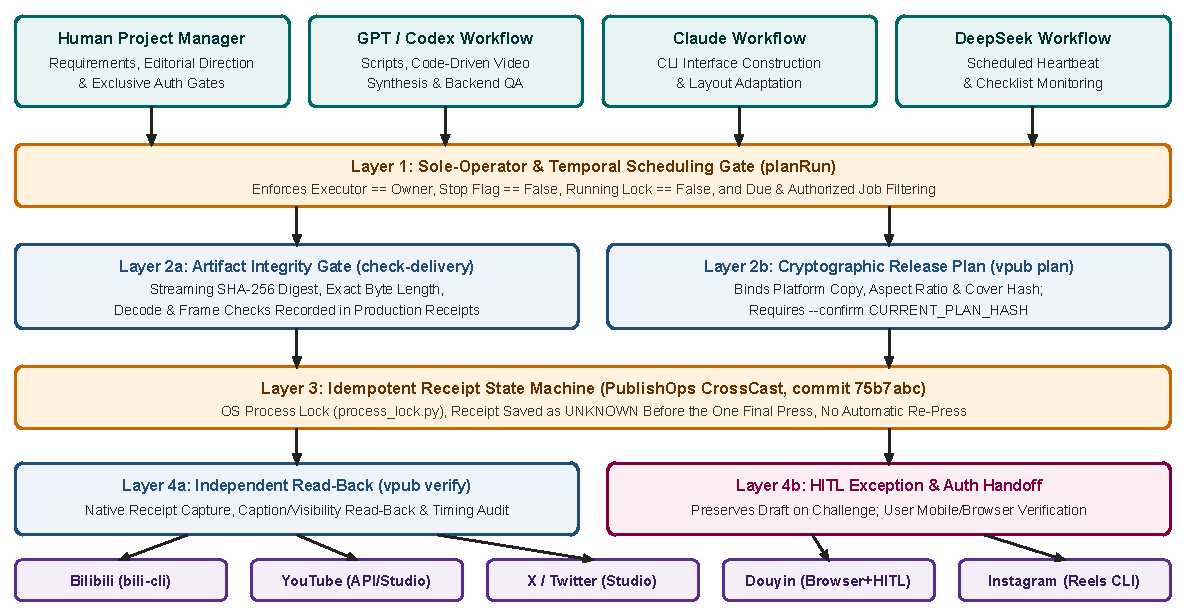
\includegraphics[width=\textwidth]{figures/fig1.pdf}
\caption{The four-layer human--AI collaborative project governance and multi-platform release architecture implemented in \emph{Agentic Work Lab} and \emph{PublishOps CrossCast}.}
\label{fig:1}
\end{figure}

\subsection{Multi-Agent Role Allocation and Handoff Boundaries}
\label{sec:4.1}

Within the laboratory environment, project execution is partitioned across four distinct actors: the Human Project Manager and three specialized AI agent workflows (GPT/Codex, Claude, and DeepSeek). Rather than allowing agents to communicate via unstructured conversational loops, all inter-agent handoffs are mediated through version-controlled state files (\texttt{operations-\allowbreak{}checklist.\allowbreak{}md}, \texttt{delivery-manifest.json}, and \texttt{production-\allowbreak{}update-\allowbreak{}*.\allowbreak{}json}). Table 2 defines the task scope, handoff artifacts, and operational constraints for each actor.

\begin{table}[htbp]
\centering
\caption{Multi-agent role allocation, handoff artifacts, and governance boundaries across the project lifecycle.}
\label{tab:2}
\scriptsize
\setlength{\tabcolsep}{3pt}
\begin{tabular}{>{\raggedright\arraybackslash}p{0.170\textwidth}>{\raggedright\arraybackslash}p{0.246\textwidth}>{\raggedright\arraybackslash}p{0.256\textwidth}>{\raggedright\arraybackslash}p{0.275\textwidth}}
\toprule
\textbf{Project Actor} & \textbf{Assigned Functional Scope} & \textbf{Observable Evidence \& Handoff Artifacts} & \textbf{Enforced Governance \& Safety Constraints} \\
\midrule
\textbf{Human Project Manager}\newline (Sole Operator / Architect) & Requirements definition, editorial direction, creative acceptance, platform authentication, and final release authorization. & Explicit authorization events (\texttt{USER\_AUTHORIZED\_*}), mobile/browser verification receipts, and plan confirmation hashes. & Retains exclusive sign-off on public releases, deletions, and schedule overrides; resolves \texttt{UNKNOWN} platform states. \\
\textbf{GPT / Codex Workflow}\newline (Production \& Backend QA) & Topic/merchant research, script synthesis, programmable video timeline assembly, FFmpeg encoding checks, and backend repository review. & SHA-256 verified \texttt{.mp4} exports, frame-sampling logs, decode error counts, and pull request verification records. & Cannot self-authorize public platform writes; unapproved or in-progress renders (\texttt{RENDER\_OR\_QA\_PENDING}) are excluded from release. \\
\textbf{Claude Workflow}\newline (Interface \& Tool Construction) & CLI interface construction, layout adaptation, portrait cut tooling, and developer user-experience refinements in \emph{CrossCast}. & Interface and first-run changes in scoped pull requests (e.g., PRs 8--10) with unit tests; commit metadata does not record which model authored a change. & Changes remain commit-scoped until verified by regression suites; local mock tests are never reported as live speedups. \\
\textbf{DeepSeek Workflow}\newline (Scheduled Operations Monitor) & Hourly automated heartbeat inspections, reading operational checklists, checking due times, and synchronizing user instructions. & Machine-readable execution traces (\texttt{scheduled-\allowbreak{}run-\allowbreak{}evidence.\allowbreak{}json}) and de-identified event logs (\texttt{operations-events.json}). & Strictly read-only when no authorized task is due; forbidden from launching duplicate runs or retrying uncertain submissions. \\
\bottomrule
\end{tabular}
\end{table}

Model names denote workflow roles: the records do not authenticate the model version behind each request (\texttt{docs/\allowbreak{}model-\allowbreak{}workflow\_\allowbreak{}EN.\allowbreak{}md}), and the 3 November record describes the person as setting requirements and acceptance, Claude as supporting construction and interfaces, and Codex as leading backend review and final repository updates.

\subsection{Layer 1: Deterministic Sole-Operator and Temporal Scheduling Gate}
\label{sec:4.2}

To prevent race conditions and unauthorized autonomous execution during scheduled heartbeats, Layer 1 enforces a pure offline decision function $\mathcal{G}_{\text{plan}}$ before any network or platform adapter is invoked. Let $\mathcal{S}$ = ($e$, $o$, $f_{\text{stop}}$, $f_{\text{run}}$, $t_{\text{now}}$, $\mathcal{J}$) denote the operational context tuple, where $e$ is the requesting executor identifier, $o$ is the registered instance owner, $f_{\text{stop}}$ $\in$ \{true, false\} is the emergency halt flag, $f_{\text{run}}$ $\in$ \{true, false\} indicates whether an execution lock is active, $t_{\text{now}}$ $\in$ $\mathbb{R}^{+}$ is the current epoch timestamp, and $\mathcal{J}$ = \{$j_{\text{1}}$, \ldots{}, $j_{m}$\} is the set of candidate jobs.

\begin{equation}
\mathcal{G}_{\text{plan}}(\mathcal{S}) =
\begin{cases}
(\texttt{skip}, \texttt{not\_owner}, \emptyset) & \text{if } e = \varnothing \lor e \neq o, \\
(\texttt{skip}, \texttt{stop\_flag}, \emptyset) & \text{else if } f_{\text{stop}} = \text{true}, \\
(\texttt{skip}, \texttt{already\_running}, \emptyset) & \text{else if } f_{\text{run}} = \text{true}, \\
(\texttt{plan\_only}, \texttt{checked}, \mathcal{D}) & \text{else if } \mathcal{D} \neq \emptyset, \\
(\texttt{no\_work\_due}, \texttt{checked}, \emptyset) & \text{otherwise},
\end{cases}
\label{eq:planrun}
\end{equation}

where the due set $\mathcal{D}$ is strictly filtered as:

\begin{equation}
\mathcal{D} = \left\{ \text{id}_k \;\middle|\; j_k \in \mathcal{J} \;\land\; \text{done}_k = \text{false} \;\land\; \text{auth}_k = \text{true} \;\land\; t_{\text{due},k} \le t_{\text{now}} \right\}
\label{eq:dueset}
\end{equation}

Furthermore, for any automated run record $R$ = (trig, status, $f_{\text{manual}}$, $t_{\text{start}}$, $t_{\text{end}}$, $E_{\text{err}}$), post-execution verification $\mathcal{V}_{\text{sched}}$($R$) holds if and only if:

\begin{equation}
\begin{aligned}
\mathcal{V}_{\text{sched}}(R) \iff\;& (\text{trig} = \texttt{automation\_heartbeat\_scheduled}) \\
&\land (\text{status} = \texttt{VERIFIED\_AUTOMATIC\_RUN\_COMPLETED}) \\
&\land (f_{\text{manual}} = \text{false}) \land (t_{\text{start}}, t_{\text{end}} \text{ finite}) \land (t_{\text{start}} \le t_{\text{end}}) \land (|E_{\text{err}}| = 0)
\end{aligned}
\label{eq:verify_sched}
\end{equation}

\begin{algorithm}[htbp]
\caption{Deterministic Sole-Operator \& Temporal Scheduling Gate (\texttt{planRun} \& \texttt{verifyScheduledRun})}
\label{alg:planrun}
\footnotesize
\begin{algorithmic}[1]
\Require Context tuple $\mathcal{S} = (e, o, f_{\text{stop}}, f_{\text{run}}, t_{\text{now}}, \mathcal{J})$; run trace record $R$
\Ensure Gate decision tuple $(\text{decision}, \text{reason}, \mathcal{D})$ and boolean verification result $v$
\State $t_{\text{cur}} \gets \text{ParseEpoch}(t_{\text{now}})$
\If{$\neg \text{IsFinite}(t_{\text{cur}})$} \textbf{throw} \texttt{Error("Invalid current time")} \EndIf
\If{$e = \varnothing \lor e \neq o$} \Return $(\texttt{"skip"}, \texttt{"not\_owner"}, \emptyset)$ \EndIf
\If{$f_{\text{stop}} = \text{true}$} \Return $(\texttt{"skip"}, \texttt{"stop\_flag"}, \emptyset)$ \EndIf
\If{$f_{\text{run}} = \text{true}$} \Return $(\texttt{"skip"}, \texttt{"already\_running"}, \emptyset)$ \EndIf
\State $I_{\text{seen}} \gets \emptyset$; $\mathcal{D} \gets [\,]$
\ForAll{$j_k = (\text{id}_k, t_{\text{due},k}, \text{auth}_k, \text{done}_k) \in \mathcal{J}$}
    \If{$\text{id}_k = \varnothing \lor \text{id}_k \in I_{\text{seen}}$} \textbf{throw} \texttt{Error("Missing or duplicate job id")} \EndIf
    \State $I_{\text{seen}} \gets I_{\text{seen}} \cup \{\text{id}_k\}$
    \If{$\text{done}_k = \text{true} \lor \text{auth}_k \neq \text{true}$} \textbf{continue} \EndIf
    \State $t_{\text{at}} \gets \text{ParseEpoch}(t_{\text{due},k})$
    \If{$\neg \text{IsFinite}(t_{\text{at}})$} \textbf{throw} \texttt{Error("Invalid due time for " + id\_k)} \EndIf
    \If{$t_{\text{at}} \le t_{\text{cur}}$} $\text{Append}(\mathcal{D}, \text{id}_k)$ \EndIf
\EndFor
\State $\text{decision} \gets (|\mathcal{D}| > 0)\ ?\ \texttt{"plan\_only"} : \texttt{"no\_work\_due"}$
\State \Return $(\text{decision}, \texttt{"checked"}, \mathcal{D})$
\end{algorithmic}
\end{algorithm}

As formalized in Algorithm 1, \texttt{planRun} is a side-effect-free admission filter. It first checks that the reference clock parses to a finite epoch value (lines 1--2), then applies three ordered circuit breakers: executor ownership (line 3), the stop flag (line 4) and the running lock (line 5). Only when all three pass does it scan the candidate jobs, rejecting missing or repeated identifiers (lines 6--9) and skipping jobs that are completed or lack explicit human authorization (line 10). Even when due jobs exist, it returns \texttt{plan\_only} rather than acting, leaving content checks and confirmation to the later layers. Two properties of the implementation (\texttt{scripts/\allowbreak{}operations-\allowbreak{}gate.\allowbreak{}mjs}) matter for interpretation. A non-finite due time raises an error only for jobs that are authorized and not completed, because other jobs are skipped before their due time is parsed. And \texttt{planRun} is advisory: it returns a decision but cannot stop an agent that never calls it. In the laboratory the operations checklist requires the call; enforcement at the platform boundary comes from Layers 2 and 3, which sit inside the release command itself.

\subsection{Layer 2: Plan-Hash Binding and Artifact Verification}
\label{sec:4.3}

Between plan approval and execution, an agent or background process may change a video export, swap a cover or alter platform copy after the project manager has reviewed the preview. Large deliverables (2.6 MB to 285.9 MB in our archive) can also be written incompletely or misread; the release record of the v3 film notes one earlier local read discrepancy that remains unexplained. Layer 2 closes this time-of-check-to-time-of-use gap with two invariants:

\begin{invariant}[Media Integrity]
Let $M = \{m_1, \dots, m_K\}$ be the release manifest, where each entry $m_i = (\text{fname}_i, B_i, H_i)$ gives a file name, an exact byte length $B_i$ and an expected SHA-256 digest $H_i$. An artifact $f_i$ passes the delivery check if and only if $\text{basename}(\text{fname}_i) = \text{fname}_i \land \text{size}(f_i) = B_i \land \text{SHA256}(f_i) = H_i$. Decode and frame checks are recorded separately in production receipts.
\end{invariant}

\begin{invariant}[Plan-Hash Confirmation Binding]
Before any platform write through \texttt{vpub publish}, the release plan $P$---target platforms, account identities, video and cover SHA-256 digests, aspect ratio, visibility and platform copy---is serialized as JSON with sorted keys and compact separators and hashed, $H(P) = \text{SHA256}(\text{CanonicalJSON}(P))$. Execution is refused unless the command supplies \texttt{--confirm}~$H_{\text{user}}$ with $H_{\text{user}} = H(P)$; a changed plan has a new digest, so a stale code is refused.
\end{invariant}

Both \texttt{check-delivery.mjs} (Node.js) and \texttt{vpub} (Python) hash media in streamed chunks rather than loading whole files, and the delivery check rejects manifest names that are not plain file names. The manifest records a zero-error full decode for five of the 30 deliveries (entries 26--30); update notes record decode checks for several others. The plan digest also names the receipt file---one per plan and platform---so a second attempt at the same plan finds the first attempt's receipt instead of starting afresh (Section 4.4). Invariant 2 binds the command to the exact content that was reviewed; it does not authenticate who approved it. The CLI records \texttt{-{}-person-approved} as the caller's attestation and states that it cannot verify who supplied it, so human authority rests on procedure (the agent must stop and show the plan) while the digest guarantees that what runs is what was shown. Loudness, clipping, silence-window and frame-scan measurements that accompany deliveries are reported per case in Table 8.

\subsection{Layer 3: Idempotent Receipt State Machine and UNKNOWN-State Suppression}
\label{sec:4.4}

To answer \textbf{RQ2}, we model each browser publication attempt in \emph{PublishOps CrossCast} as a durable receipt whose changes are written atomically under a file lock, while cross-process OS locks (\texttt{process\_lock.py}) keep two runs from driving the same browser profile (Figure 2, Algorithm 2). The receipt is stored at a path named by the plan digest and the platform and holds $\mathcal{R}_p$ = (key, $\text{acct}_{p}$, $H_{\text{media}}$, $H_{\text{meta}}$, $f_{\text{submit}}$, $\sigma_{p}$, $\text{wid}_{p}$, $\tau_{\text{log}}$), where $f_{\text{submit}}$ is the implementation's \texttt{final\_submit\_attempted} field and $\sigma_{p}$ its state. Before pressing, the receipt also records the account's existing work identifiers, so that read-back can later look for exactly one new work. Figure 2 shows the states used at commit \texttt{75b7abc} (\texttt{browser\_backends.py}).

\begin{figure}[htbp]
\centering
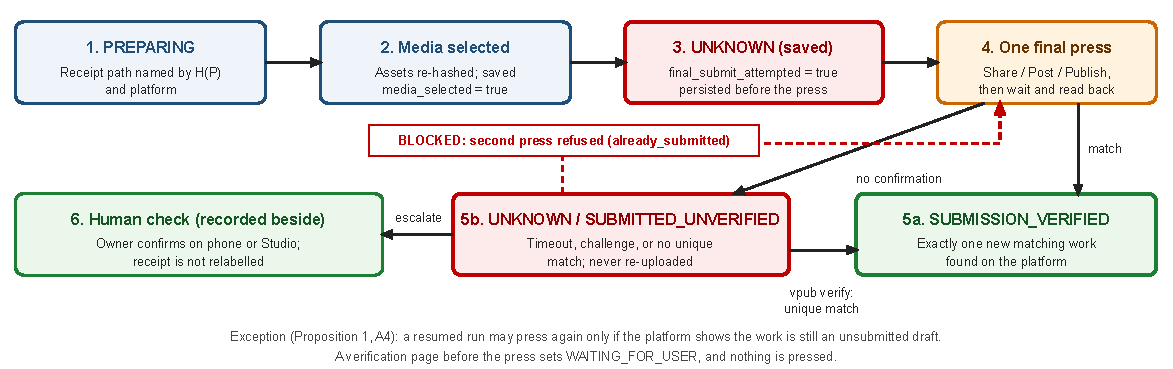
\includegraphics[width=\textwidth]{figures/fig2.pdf}
\caption{Receipt states of a browser publication attempt in \emph{PublishOps CrossCast} (commit \texttt{75b7abc}). The receipt is saved as \texttt{UNKNOWN} with \texttt{final\_\allowbreak{}submit\_\allowbreak{}attempted = true} before the single final press; a later run refuses a second press unless the platform shows the work is still a draft, and only read-back or a person settles the outcome.}
\label{fig:2}
\end{figure}

\begin{algorithm}[htbp]
\caption{Idempotent Cross-Platform Publication \& \texttt{UNKNOWN}-State Latching (\texttt{vpub publish} \& \texttt{vpub verify})}
\label{alg:publish}
\footnotesize
\begin{algorithmic}[1]
\Require Release plan $P$ with digest $H(P)$, confirmation code $H_{\text{user}}$, platform $p$, account $\text{acct}_p$, resume flag
\Ensure Persistent receipt $\mathcal{R}_p = (\text{key}, \text{acct}_p, H_{\text{media}}, H_{\text{meta}}, f_{\text{submit}}, \sigma_p, \text{wid}_p, \tau_{\text{log}})$
\If{$H_{\text{user}} \neq H(P)$} \textbf{abort} (stale or wrong plan code) \EndIf
\State $\text{AcquireProcessLock}(p, \text{acct}_p)$ \Comment{a stale lock is taken over only after its owner process has exited}
\State $\text{path} \gets \text{ReceiptPath}(H(P), p)$
\If{$\text{Exists}(\text{path}) \land \neg\text{resume}$} \textbf{abort} \texttt{attempt\_exists} \Comment{never reset an attempt to upload again} \EndIf
\If{$\text{resume} \land \text{Exists}(\text{path})$} $\mathcal{R}_p \gets \text{Load}(\text{path})$; require the same $H_{\text{media}}$ and $\text{acct}_p$, else \textbf{abort} \texttt{receipt\_conflict} \EndIf
\If{$\text{resume} \land \neg\text{Exists}(\text{path})$ and the publication record shows media selected or a press attempted} \textbf{abort} \texttt{receipt\_missing} \EndIf
\State $\text{VerifySHA256}(P.\text{media}, P.\text{covers})$; select media; $\mathcal{R}_p.\text{media\_selected} \gets \text{true}$; $\text{PersistAtomically}(\mathcal{R}_p)$
\If{$\mathcal{R}_p.f_{\text{submit}} = \text{true} \land \neg\text{PlatformShowsUnsubmittedDraft}()$} \textbf{abort} \texttt{already\_submitted} \EndIf
\State $\mathcal{R}_p.\sigma_p \gets \texttt{UNKNOWN}$; $\mathcal{R}_p.f_{\text{submit}} \gets \text{true}$; $\text{PersistAtomically}(\mathcal{R}_p)$ \Comment{before the click}
\State $\text{PressFinalSubmitOnce}()$ \Comment{a single Share / Post / Publish press}
\State $\text{outcome} \gets \text{AwaitConfirmationAndReadBack}(\text{acct}_p, \text{new works not listed before the press})$
\If{outcome holds exactly one matching new work} $\mathcal{R}_p.\sigma_p \gets \texttt{SUBMISSION\_VERIFIED}$; $\mathcal{R}_p.\text{wid}_p \gets \text{outcome}.\text{work\_id}$
\Else\ keep $\mathcal{R}_p.\sigma_p \in \{\texttt{UNKNOWN}, \texttt{SUBMITTED\_UNVERIFIED}\}$ \Comment{never re-press; escalate to \texttt{vpub verify} or a person}
\EndIf
\State $\text{PersistAtomically}(\mathcal{R}_p)$; $\text{ReleaseProcessLock}(p, \text{acct}_p)$; \Return $\mathcal{R}_p$
\end{algorithmic}
\end{algorithm}

\begin{proposition}[At-Most-Once Automated Final Submission]
\label{prop:idempotency}
Assume (A1) every final submission for plan $P$ on platform $p$ goes through the receipt transaction of Algorithm~\ref{alg:publish}; (A2) receipt writes are atomic and durable; and (A3) receipts are not edited by hand. Then automated runs issue at most one final press per $(P, p)$, with one exception: (A4) a resumed run may press again when the platform shows that the earlier work is still an unsubmitted draft.
\end{proposition}
\begin{proof}[Proof sketch]
The receipt is saved with $\sigma_p = \texttt{UNKNOWN}$ and $f_{\text{submit}} = \text{true}$ before the press (line~9). A later run on the same plan either finds the receipt and stops (line~4) or resumes it, in which case line~8 refuses another press while $f_{\text{submit}} = \text{true}$ unless (A4) holds. If the receipt file has disappeared while the publication record shows a selected file or an attempted press, the run stops (line~6) instead of uploading again.
\end{proof}

Proposition 1 is a safety guarantee, not a liveness one. A crash between saving the receipt and pressing leaves an \texttt{UNKNOWN} receipt for a submission that never happened; the design accepts such false alarms because the opposite error, a duplicate public post, cannot be undone. Whether an \texttt{UNKNOWN} submission published is settled afterwards by \texttt{vpub verify}, which checks that the signed-in account is the receipt's account and upgrades the receipt only when it finds exactly one matching new work, or by a person whose confirmation is recorded beside the receipt without relabelling it. Resumable byte offsets belong to API routes (\texttt{upload\_resume.py} in the laboratory's 0.15.1 snapshot); the browser route instead refuses to upload again once its record shows that a file was selected.

\subsection{Layer 4: Identity-Bound In-Place Revision and Consent-Bound Deletion}
\label{sec:4.5}

Beyond first publication, channel operations revise captions and covers, assign chapters and occasionally delete test works. An agent that implements an edit as delete-and-repost, or deletes without confirming the target's identity, turns a reversible correction into an irreversible loss. Layer 4 binds every revision and deletion to the receipt's account and work identifier (Algorithm 3), developed across PRs \#20, \#21, \#25, \#29 and \#30.

\begin{algorithm}[htbp]
\caption{Identity-Bound In-Place Revision \& Consent-Bound Single-Work Deletion (\texttt{vpub edit} \& \texttt{vpub delete})}
\label{alg:editdelete}
\footnotesize
\begin{algorithmic}[1]
\Require Receipt key $K$, patch $\Delta P$ or deletion request, mode $\in \{\texttt{VERIFY\_ONLY}, \texttt{APPLY\_EDIT}, \texttt{DELETE\_WORK}\}$
\Ensure Edit or deletion state and audit entry
\State $\mathcal{R}_p \gets \text{LoadReceipt}(K)$; require the signed-in account $= \mathcal{R}_p.\text{acct}_p$ (\texttt{expected\_identity})
\If{$\text{mode} \in \{\texttt{VERIFY\_ONLY}, \texttt{APPLY\_EDIT}\}$}
    \State $\text{live} \gets \text{ReadNativeEditorFields}(\mathcal{R}_p.\text{wid}_p)$ \Comment{page translations and comments are ignored}
    \If{$\text{live} = \Delta P.\text{target}$} \Return \texttt{EDIT\_VERIFIED} \Comment{nothing to save} \EndIf
    \If{$\text{mode} = \texttt{VERIFY\_ONLY}$} \Return \texttt{EDIT\_MISMATCH} \EndIf
    \If{the platform offers no in-place edit for this work} \Return \texttt{EDIT\_UNAVAILABLE} \Comment{never delete or repost instead} \EndIf
    \State checkpoint \texttt{EDIT\_PREPARING}; $\text{ApplyInPlace}(\mathcal{R}_p.\text{wid}_p, \Delta P)$ \Comment{video bytes and visibility unchanged}
    \State reopen the editor; \Return \texttt{EDIT\_VERIFIED} if read-back equals $\Delta P.\text{target}$, else \texttt{EDIT\_SUBMITTED\_UNVERIFIED}
\ElsIf{$\text{mode} = \texttt{DELETE\_WORK}$}
    \State require a dry run and a person's approval of this exact work (\texttt{--confirm} code, \texttt{--person-approved}), stored durably
    \State wait until the deletion control is ready; $\text{DeleteSingleWork}(\mathcal{R}_p.\text{wid}_p)$
    \State refresh the catalogue; report success only if the work is absent
\EndIf
\end{algorithmic}
\end{algorithm}

Algorithm 3 adds three safeguards. First, every read or change begins by confirming that the active session belongs to the receipt's account (\texttt{expected\_identity}), preventing cross-account changes. Second, an edit compares native editor fields rather than the rendered page, and where the platform offers no in-place edit---as for an X post whose menu has no Edit action---the run ends with \texttt{EDIT\_UNAVAILABLE} and attempts no deletion, repost or reply: compensation by repost would lose the post's identifier, replies and reach (Section 2.4). Third, a deletion requires a dry run and a person's approval of that exact work, waits until the deletion control is ready (PR \#30), and counts as done only when a refreshed catalogue no longer lists the work (PR \#29).

\section{System Implementation: Agentic Work Lab and PublishOps CrossCast}
\label{sec:5}

\subsection{Programmable Video Synthesis and Multi-Modal Quality Gates}
\label{sec:5.1}

Within \emph{Agentic Work Lab}, video production is engineered as an editable, code-driven workflow (\texttt{editable-\allowbreak{}video-\allowbreak{}workflow.\allowbreak{}md}) rather than opaque one-shot video generation. Audio narration timelines, character pose transitions, camera movements, and bilingual subtitles are defined programmatically so that localized defects can be repaired in place without regenerating unaffected segments (Figure 3).

\begin{figure}[htbp]
\centering
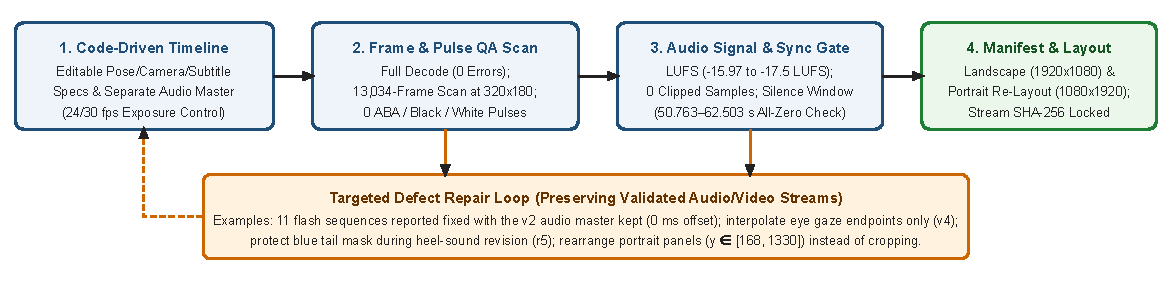
\includegraphics[width=\textwidth]{figures/fig3.pdf}
\caption{The programmable video synthesis and multi-modal quality verification pipeline in \emph{Agentic Work Lab} (values from the delivery records summarized in Table 8).}
\label{fig:3}
\end{figure}

\subsection{CrossCast Two-Slot Concurrent Browser Architecture and Session Reuse}
\label{sec:5.2}

\emph{PublishOps CrossCast} was released publicly as \texttt{v0.16.0} (commit \texttt{a46bd19}) and developed on its main branch to commit \texttt{75b7abc} (PR \#30, 3 November 2026), the snapshot evaluated here. At that commit the repository holds 123 Python source files (26,972 physical lines): 81 files (18,005 lines) form \emph{CrossCast}'s own package, and 42 files (8,967 lines) are an unmodified copy of the MIT-licensed \texttt{bili-cli} v1.2.1, bundled for Bilibili access (\texttt{NOTICE.md}). Its 126 test files (122 test modules and four shared helpers; 37,029 lines) define 2,737 test functions, up from 2,009 in 84 files at \texttt{v0.16.0}, and GitHub's continuous-integration checks for \texttt{75b7abc} passed on Python 3.10--3.14. Because one Instagram run spent most of its time waiting after submission (Table 7), PRs \#11 and \#15 (\texttt{066c49f}, \texttt{6f7b62b}) added a bounded two-slot scheduler for browser platforms (Figure 4): each platform keeps its own account lock, browser session and receipt, up to two browser platforms publish at once, and the next queued platform starts when a slot frees. No concurrent publication has yet been timed, so no speedup is claimed. API routes for YouTube, X and Instagram are distributed separately from the public repository and lie outside the evaluated snapshot.

\begin{figure}[htbp]
\centering
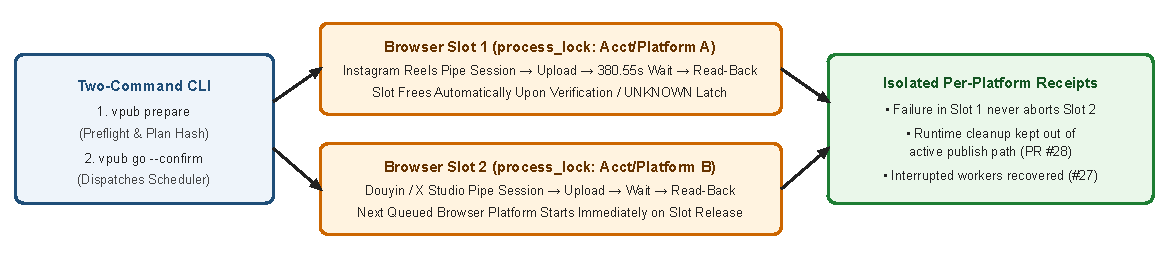
\includegraphics[width=\textwidth]{figures/fig4.pdf}
\caption{Two-command release workflow (\texttt{prepare}/\texttt{go}) and bounded two-slot concurrent browser publication in \emph{PublishOps CrossCast} (PRs \#10, \#11, \#15, \#27, \#28). Architecture only: the Instagram wait shown in Slot 1 comes from a sequential run, and no concurrent run has been timed.}
\label{fig:4}
\end{figure}

\section{Empirical Evaluation and Results}
\label{sec:6}

\subsection{Operational Journal and Write Evidence (RQ1)}
\label{sec:6.1}

The operational journal (\texttt{data/\allowbreak{}operations-\allowbreak{}events.\allowbreak{}json}) is an export of selected fields from the laboratory's local event logs. It holds 69 records, of which 46 are timestamped, between 26 October 01:27 and 27 October 02:45 (UTC+8, a 25.3-hour window); it was exported on 28 October. Because the export kept different fields for different records---33 carry an event name, 5 only a state name and 31 neither---we classify the records by the write evidence each one carries rather than by a coding of their purpose (Table 3).

\begin{table}[htbp]
\centering
\caption{Write evidence in the $N$ = 69 records of the operational journal, classified by the fields each record carries (recomputed by \texttt{reproduce\_\allowbreak{}paper\_\allowbreak{}tables.\allowbreak{}mjs}).}
\label{tab:3}
\scriptsize
\setlength{\tabcolsep}{3pt}
\begin{tabular}{>{\raggedright\arraybackslash}p{0.285\textwidth}>{\raggedleft\arraybackslash}p{0.074\textwidth}>{\raggedleft\arraybackslash}p{0.083\textwidth}>{\raggedleft\arraybackslash}p{0.083\textwidth}>{\raggedleft\arraybackslash}p{0.083\textwidth}>{\raggedright\arraybackslash}p{0.313\textwidth}}
\toprule
\textbf{Evidence Carried by the Record} & \textbf{Records} & \textbf{Share} & \textbf{Platform Reads} & \textbf{Platform Writes} & \textbf{What the Record Shows} \\
\midrule
Explicit zero-write field (\texttt{platform\_writes}, \texttt{write\_calls} or \texttt{platform\_write\_calls} = 0) & 20 & 28.99\% & 13 & 0 & States that no write occurred; includes the four read-only sampling runs (26 CLI calls) and the four automation-triggered checks. \\
Zero platform calls (\texttt{platform\_calls} = 0; no write field) & 39 & 56.52\% & 0 & 0 & No platform call, hence no write. \\
One platform call, no write field (record 22) & 1 & 1.45\% & --- & --- & Event name indicates a sign-in check after a title choice; reads and writes not recorded. \\
One platform write (record 52) & 1 & 1.45\% & 4 & 1 & Unnamed in the export; four reads recorded with it; \texttt{new\_risk} = false. \\
No call or write field & 8 & 11.59\% & --- & --- & Silent on writes; the absence of a write is not shown. \\
\midrule
\textbf{Total} & \textbf{69} & \textbf{100.00\%} & \textbf{17} & \textbf{1} & \textbf{No record reports a replayed upload.} \\
\bottomrule
\end{tabular}
\end{table}

Table 3 supports three statements and rules out a fourth. (i) One record reports a platform write (record 52: one write and four reads, \texttt{new\_risk} = false); the export does not name the action. (ii) No record reports a replayed upload: the replay counter appears in one record (value 0), and all eight records that carry \texttt{new\_risk} report false. (iii) 59 records carry an explicit zero count of writes or platform calls; the other nine are silent on writes. What the journal cannot show is that a gate blocked an attempted write: it records outcomes, not refused attempts, so the absence of writes in 68 records is consistent with, but not evidence of, suppression. Evidence that Layer 1 makes the intended decisions comes instead from the four automation-triggered records (all without writes and with the stop flag off), the heartbeat trace below, and the workflow tests (10/10 passed, \texttt{results/\allowbreak{}validation.\allowbreak{}json}).

The audited DeepSeek heartbeat (\texttt{scheduled-\allowbreak{}run-\allowbreak{}evidence.\allowbreak{}json}, planned for \texttt{2026-\allowbreak{}10-\allowbreak{}28T12:37:13.\allowbreak{}943+08:00}) started after a delay of 24,992 ms (24.992 s) and completed its four recorded work items---reading ownership, checklist, stop conditions and checkpoints; finding no comment, component, research or analytics work due; synchronizing instructions; and needing no Bilibili operation---in 31,175 ms (31.175 s), with no task errors, no manual test trigger and no duplicate run. The record satisfies $\mathcal{V}_{\text{sched}}$ (Eq. 3).

\subsection{Software Verification and Design Science Evolution (RQ1 \& RQ2)}
\label{sec:6.2}

Live experiments must not pollute public accounts with deliberate faults such as double posting or deleting production videos, so offline tests are the main evidence for edge-case transitions; one live crash-recovery check was run on a private clip (Table 5). Table 4 summarizes the \emph{CrossCast} test suite at commit \texttt{75b7abc}, grouped by file name, and Table 5 traces the design iterations. Test-function counts measure the volume of checking, not coverage; no coverage tool was run.

\begin{table}[htbp]
\centering
\caption{Code and offline test volume of \emph{PublishOps CrossCast} at commit \texttt{75b7abc}, with test files grouped by file name (first matching rule; a file may exercise several concerns), and the \emph{Agentic Work Lab} entry points. Lines are physical lines.}
\label{tab:4}
\scriptsize
\setlength{\tabcolsep}{3pt}
\begin{tabular}{>{\raggedright\arraybackslash}p{0.317\textwidth}>{\raggedleft\arraybackslash}p{0.075\textwidth}>{\raggedleft\arraybackslash}p{0.093\textwidth}>{\raggedleft\arraybackslash}p{0.103\textwidth}>{\raggedright\arraybackslash}p{0.345\textwidth}}
\toprule
\textbf{Group / Entry Point} & \textbf{Files} & \textbf{Lines} & \textbf{Test Functions} & \textbf{Examples of Behaviour Exercised} \\
\midrule
\multicolumn{5}{l}{\textit{A. PublishOps CrossCast at \texttt{75b7abc} (123 source files, 26,972 lines, of which 42 files are bundled \texttt{bili-cli} v1.2.1)}} \\
1. Publishing workflow, receipts, locks \& recovery & 20 & 7,547 & 494 & Two-command \texttt{prepare}/\texttt{go} flow, publish-plan safety, worker slots and refill, checkpoint de-duplication, browser broker and lock lifecycle. \\
2. Deletion \& absence read-back & 19 & 6,830 & 340 & Consent, dialogs, loading, timelines and absence read-back for single-work deletion across platforms. \\
3. Edits \& metadata read-back & 5 & 1,615 & 128 & X edit consistency and length, Bilibili mention links, staged edits. \\
4. Platform pages \& adapters & 20 & 7,154 & 590 & YouTube Studio, X site and schedules, Douyin forms, Instagram media and comments. \\
5. Collections \& playlists & 8 & 2,792 & 259 & Collection membership, page redraws, empty and incomplete playlists. \\
6. Messages, comments, engagement \& safety & 18 & 4,300 & 402 & Comment snapshots, replies, likes, hostile-message flags and rate limits. \\
7. Other CLI, documentation \& installation & 32 & 6,383 & 524 & Capabilities, first run, preferences, covers, installer and documentation checks. \\
\midrule
\textbf{Subtotal (incl. 4 shared helper files, 408 lines)} & \textbf{126} & \textbf{37,029} & \textbf{2,737} & \textbf{Test-to-source line ratio 1.37 (2.06 against \emph{CrossCast}'s own 18,005-line package).} \\
\addlinespace
\multicolumn{5}{l}{\textit{B. Agentic Work Lab Entry Points (Node.js v26.11.1)}} \\
8. Workflow gate \& merchant demo (\texttt{workflows.test.mjs}) & 1 & 27 & 10 & Non-owner rejection, stop flag, running lock, invalid due time, scheduled-run verification (10/10 passed; \texttt{results/\allowbreak{}validation.\allowbreak{}json}, 28 Oct). \\
9. Archive integrity record (\texttt{media/manifest.json}) & 1 & --- & 30 records & Size and SHA-256 of 30 GitHub assets recorded as verified on 3 Nov; \texttt{SHA256SUMS.txt} matches the manifest. \\
\bottomrule
\end{tabular}
\end{table}

\begin{table}[htbp]
\centering
\caption{Design Science evolution of \emph{PublishOps CrossCast} from early prototypes to commit \texttt{75b7abc} (PR \#30).}
\label{tab:5}
\scriptsize
\setlength{\tabcolsep}{3pt}
\begin{tabular}{>{\raggedright\arraybackslash}p{0.170\textwidth}>{\raggedright\arraybackslash}p{0.246\textwidth}>{\raggedright\arraybackslash}p{0.265\textwidth}>{\raggedright\arraybackslash}p{0.265\textwidth}}
\toprule
\textbf{Version / Commit} & \textbf{Architectural Milestone} & \textbf{Empirical \& CI Verification Evidence} & \textbf{Identified Boundary \& Subsequent DSR Refinement} \\
\midrule
\texttt{v0.2.2-{}-v0.3.0}\newline (lab commit \texttt{596e951}) & Initial 5-platform adapters, X Media Studio 16:9 thumbnail persistence, FFmpeg 79.5s cover-lead synthesis. & 86 offline tests passed; verified YouTube Studio category change \& 1,327-char Instagram caption read-back. & Instagram profile grid cropped landscape cover text; TikTok suspended after a sign-in with a Hong Kong (+852) number failed. \\
\texttt{v0.15.1}\newline (Lab Snapshot) & OS process lock (\texttt{process\_lock.py}), private pipe browser context reuse, resumable byte-offset recovery. & 417 offline tests passed; a private YouTube upload forced to exit after 8,388,608 acknowledged bytes resumed in a second process and kept the same video ID (30 Oct). & Needed independent CI matrix verification and stricter schedule/pin counterexample checks. \\
Candidates\newline \texttt{eaa1aab} / \texttt{80e166b} / \texttt{2d54c8f} & Separated development from independent validation; tested X schedule submission and cleanup. & GitHub CI passed on Python 3.10--3.12; 143 + 16 targeted local checks passed; X temp media deleted \& confirmed absent. & Counterexample found imprecise pinned-comment ID (live pin held); X schedule row lacked post/media ID pair (kept \texttt{SUBMITTED\_UNVERIFIED}). \\
\texttt{v0.16.0} Release\newline (\texttt{a46bd19} / PR \#8--\#9) & Public standalone CLI release; shortened default capability list (\texttt{-{}-full}) and separated rehearsal from live readiness. & Suite of 2,009 test functions in 84 files at \texttt{a46bd19}. Field release of \emph{I Watched It For You (v3)} on 2--3 Nov with one instrumented Instagram run (412.217 s); the release record does not name the code version used per platform. & Post-submit wait consumed 92.32\% of publish time; motivated explicit wait progress and bounded concurrency. \\
PRs \#10--\#28\newline (\texttt{d97835f}--\texttt{439c038}) & Two-command \texttt{prepare}/\texttt{go} flow (\#10), two-slot browser concurrency (\#11/\#15), YouTube single-Save guard (\#16), X edit consistency (\#21). & Python 3.13/3.14 support (\#14); prompt login return \& interrupted worker recovery (\#27); runtime cleanup isolated (\#28). & Required durable consent and post-deletion absence read-back for single-work deletions across all platforms. \\
PRs \#29--\#30\newline (\texttt{3b56bdc} / \texttt{75b7abc}) & Durable-consent single-work deletion with absence read-back (\#29); deletion control readiness \& layout guards (\#30). & Suite at \textbf{126 test files (37,029 lines, 2,737 test functions)}; GitHub CI checks passed on Python 3.10--3.14. & Live multi-platform concurrent speedup benchmarking scheduled as next empirical evaluation phase. \\
\bottomrule
\end{tabular}
\end{table}

\subsection{Cross-Platform Release Verification and Latency Bottleneck Analysis (RQ2 \& RQ3)}
\label{sec:6.3}

To examine the release layers under real platform conditions, we use the release of the 176.4 s short film \emph{I Watched It For You (v3)} (\texttt{i-\allowbreak{}watched-\allowbreak{}it-\allowbreak{}for-\allowbreak{}you-\allowbreak{}v3-\allowbreak{}20261102.\allowbreak{}mp4}, 285,855,005 bytes, SHA-256 \texttt{7d6fd76090f7\allowbreak{}a93b2711e15d\allowbreak{}b4bb924f741d\allowbreak{}3a904a01fc4b\allowbreak{}7628fc2130db\allowbreak{}afdc}) on five platforms on 2--3 November 2026 (Table 6), and the phase timing recorded for its Instagram publication (Table 7, Figure 5). Each platform entry comes from its own publication run or from the owner's confirmation; the 3 November record made no fresh platform queries.

\begin{table}[htbp]
\centering
\caption{Cross-platform publication record for \emph{I Watched It For You (v3)} (\texttt{production-\allowbreak{}update-\allowbreak{}2026-\allowbreak{}11-\allowbreak{}03.\allowbreak{}json}). States are quoted as recorded; ``---'' means the record holds no such field.}
\label{tab:6}
\scriptsize
\setlength{\tabcolsep}{3pt}
\begin{tabular}{>{\raggedright\arraybackslash}p{0.103\textwidth}>{\raggedright\arraybackslash}p{0.196\textwidth}>{\raggedright\arraybackslash}p{0.159\textwidth}>{\raggedright\arraybackslash}p{0.215\textwidth}>{\raggedright\arraybackslash}p{0.261\textwidth}}
\toprule
\textbf{Platform} & \textbf{Route or Continuity (as Recorded)} & \textbf{Native Receipt State} & \textbf{Recorded Verification State} & \textbf{Outcome and Evidence} \\
\midrule
\textbf{Bilibili} & Production-session report; not re-queried (\texttt{fresh\_check} = false) & --- & \texttt{public\_\allowbreak{}reported\_\allowbreak{}by\_\allowbreak{}production\_\allowbreak{}session} (\texttt{BV15B4F6hEYr}) & Public availability recorded on 2 Nov at 21:01 UTC+8. \\
\textbf{YouTube} & Continued from the original draft & \texttt{SUBMISSION\_VERIFIED} & \texttt{PUBLIC\_VERIFIED} (\texttt{AzW6vr8nvDM}) & Native receipt, full copy and public visibility passed read-back. \\
\textbf{X} & Reused the original uploaded media & \texttt{SUBMISSION\_VERIFIED} & \texttt{PUBLIC\_VERIFIED} (\texttt{2117261340633161838}) & Receipt and 176.4 s duration verified; stored resolution not established. \\
\textbf{Douyin} & Programmatic read-back timed out & \textbf{\texttt{UNKNOWN}} & \texttt{USER\_\allowbreak{}CONFIRMED\_\allowbreak{}VISIBLE\_\allowbreak{}NATIVE\_\allowbreak{}VERIFY\_\allowbreak{}BLOCKED} & Neither relabelled nor republished; the owner's phone screenshot shows the work and production cover. \\
\textbf{Instagram} & One upload and one Share (3 Nov) & \texttt{SUBMISSION\_VERIFIED} & --- (\texttt{metadata\_readback} = true) & Full Chinese/English caption read back; original ratio; AI label on; cover replaced by the owner on mobile. \\
\bottomrule
\end{tabular}
\end{table}

The Douyin entry is the field instance of Proposition 1. The run pressed Publish once; its programmatic read-back then timed out, and the receipt kept the \texttt{UNKNOWN} state it had been given before the press. No run submitted the 285.9 MB file again, and the owner's phone confirmed that the work and its production cover were live---a confirmation recorded beside the receipt rather than written into it. A separate test on 1 November had the same shape: a Douyin scheduled card showed the requested time and private marker, the CLI read-back timed out, and the failure receipt was kept as recorded while the temporary item was removed. These are two instances, not a rate. The records do not say why read-back timed out, and the claim that a retrying agent would have published a duplicate is an inference from the retry policy (Table 11), not an observation. The Instagram row shows a second, benign use of the human channel: the owner replaced the cover on mobile, and the record notes that remote cover pixels were not verified.

\begin{table}[htbp]
\centering
\caption{Phase timing of one Instagram publication ($N$ = 1; \texttt{production-\allowbreak{}update-\allowbreak{}2026-\allowbreak{}11-\allowbreak{}03.\allowbreak{}json}). The source selects major phases rather than an exhaustive additive breakdown; row 7 is derived.}
\label{tab:7}
\scriptsize
\setlength{\tabcolsep}{3pt}
\begin{tabular}{>{\raggedright\arraybackslash}p{0.411\textwidth}>{\raggedright\arraybackslash}p{0.205\textwidth}>{\raggedleft\arraybackslash}p{0.103\textwidth}>{\raggedleft\arraybackslash}p{0.103\textwidth}>{\raggedleft\arraybackslash}p{0.112\textwidth}}
\toprule
\textbf{Execution Phase} & \textbf{Execution Scope} & \textbf{Duration (s)} & \textbf{\% of Cmd} & \textbf{\% of E2E} \\
\midrule
1. Source \& Release Plan Cryptographic Checks & Outside Publish Cmd & 0.438 & --- & 0.10\% \\
2. Local Dry-Run Rehearsal & Outside Publish Cmd & 0.444 & --- & 0.10\% \\
3. Sign-In Preflight \& Session Close & Outside Publish Cmd & 10.137 & --- & 2.40\% \\
\addlinespace
Subtotal: Pre-Publication Governance Checks & Outside Publish Cmd & 11.019 & --- & 2.60\% \\
4. Browser Start to Media File Entry & Inside \texttt{vpub publish} & 11.058 & 2.68\% & 2.61\% \\
\textbf{5. Wait after the single Share (transfer, processing \& confirmation; not separable)} & \textbf{Inside \texttt{vpub publish}} & \textbf{380.551} & \textbf{92.32\%} & \textbf{89.91\%} \\
6. Independent Post-Publication Read-Back & Inside \texttt{vpub publish} & 5.224 & 1.27\% & 1.23\% \\
7. Residual (derived: command total minus rows 4--6) & Inside \texttt{vpub publish} & 15.384 & 3.73\% & 3.63\% \\
\addlinespace
Subtotal: Publication Command Total & Inside \texttt{vpub publish} & 412.217 & 100.00\% & 97.40\% \\
\midrule
\textbf{Total End-to-End Observed Workflow Time} & \textbf{All Recorded Phases} & \textbf{423.236} & \textbf{---} & \textbf{100.00\%} \\
\bottomrule
\end{tabular}
\end{table}

\begin{figure}[htbp]
\centering
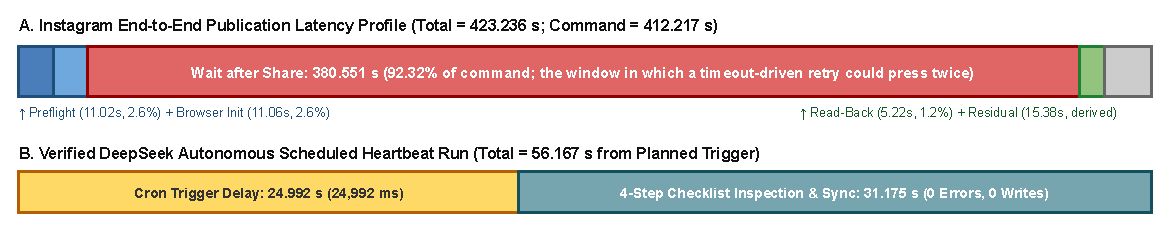
\includegraphics[width=\textwidth]{figures/fig5.pdf}
\caption{Timelines of (A) the instrumented Instagram publication run ($N$ = 1), in which the wait after the single Share made up 92.32\% of the publish command and the receipt had been saved before the press, and (B) the verified DeepSeek heartbeat run ($N$ = 1).}
\label{fig:5}
\end{figure}

\subsection{Multi-Modal Quality Engineering and Complete 30-Artifact Catalogue (RQ3)}
\label{sec:6.4}

To show how Layer 2 governs deliverable quality across revisions, Table 8 summarizes frame-level and audio measurements recorded in the production studies, and Table 9 lists all $N$ = 30 video versions archived in \emph{Agentic Work Lab} with their recorded SHA-256 digests.

\begin{table}[htbp]
\centering
\caption{Programmable video quality cases and targeted repairs, with measurements as recorded in the cited documents.}
\label{tab:8}
\scriptsize
\setlength{\tabcolsep}{3pt}
\begin{tabular}{>{\raggedright\arraybackslash}p{0.189\textwidth}>{\raggedright\arraybackslash}p{0.227\textwidth}>{\raggedright\arraybackslash}p{0.265\textwidth}>{\raggedright\arraybackslash}p{0.265\textwidth}}
\toprule
\textbf{Production Case} & \textbf{Diagnosed Technical Defect} & \textbf{Surgical Code / Timeline Repair} & \textbf{Quantitative Verification \& Documented Limits} \\
\midrule
\textbf{Animation Timing Diagnostic}\newline (\texttt{animation-timing.md}) & Changing render from 24 to 30 fps failed to create missing contact, load-transfer, and withdrawal actions. & Decomposed 24 fps exposure rules (ones = 24, twos = 12, threes = 8 exp/s) and 5-stage physical handoff criteria. & 66.7 s (2,001 frames at 30 fps): 52 segments, 44 holds (median hold 0.85 s, max 7.0 s). Established diagnostic baseline. \\
\textbf{GPT Duty Log 05}\newline (\texttt{v3-antiflash}, 434.47 s) & Full-opacity frame before fade, white flashes during right-panel changes, and shot leakage at cuts. & Set explicit hidden initial states, frame-aligned boundaries, whole-panel replacement, and 4-frame clean-entry hold; kept v2 audio. & \textbf{13,034 / 13,034 frames scanned} at 320$\times$180: 11 sequences reported fixed; 0 ABA/black/white pulses; $-$15.97 LUFS, $-$2.21 dBTP, 0 ms audio offset. \\
\textbf{Whale Girl Transformation}\newline (\texttt{v3} 67s $\rightarrow$ \texttt{v4} 75.23s) & Abrupt eye gaze jumps, brightness mismatch across cut, and moving tail fin entering fixed hair mask. & Interpolated eye regions only between real source endpoints; matched cut brightness; expanded v4 protection mask; ducked music 12 dB. & 1080$\times$1920, 2,257 frames: 0 decode errors, 0 clipped samples (sample peak $\approx$ $-$1.636 dBFS), all-zero silence verified from 50.763 to 62.503 s, black frame at 1,845 (61.500 s). \\
\textbf{Whale Girl Revisions}\newline (\texttt{r5} Colour/Heels \& \texttt{r7} Motion) & Colour spill onto blue tail during grading (r5); uneven alternating steps in sock/heart gestures (r7). & Separated clothing/skin/background masks protecting tail \& 6 heel events (r5); reordered real source frames without optical flow (r7). & r5: 66.87 s (2,006 frames), full decode passed (+1.11 dBFS inherited float peak noted). r7: 65.37 s (1,961 frames), join \& duplicate-frame checks passed. \\
\textbf{Whale Girl Ep 07 \& Portrait Cuts A/B/C}\newline (179.77 s + 3 cuts) & Cropping 1920$\times$1080 landscape to 1080$\times$1920 portrait cuts off ticket counters and character art. & Programmatically rearranged ticket/character panels into $y$ $\in$ [168, 1330] (56 px subtitles, 106 px numbers) at 360 px preview width. & 5,393 landscape frames + 843/897/899 portrait frames; portrait cuts $-$17.5/$-$16.6/$-$17.5 LUFS, peaks $\approx$ $-$1.5 dBFS, 0 clipped samples. Documented 130 ms first-ticket stamp offset vs. earlier 6 ms estimate. \\
\bottomrule
\end{tabular}
\end{table}

\begin{table}[htbp]
\centering
\caption{All $N$ = 30 downloadable video versions archived in \emph{Agentic Work Lab} (2,211,716,129 bytes; 2.21 GB or 2,109.26 MiB). GitHub asset sizes and SHA-256 digests were recorded as verified on 3 November 2026, and \texttt{SHA256SUMS.txt} matches the manifest. State: Bilibili state, current where recorded, otherwise at snapshot.}
\label{tab:9}
\tiny
\setlength{\tabcolsep}{3pt}
\begin{tabular}{>{\raggedleft\arraybackslash}p{0.036\textwidth}>{\raggedright\arraybackslash}p{0.232\textwidth}>{\raggedright\arraybackslash}p{0.241\textwidth}>{\raggedleft\arraybackslash}p{0.063\textwidth}>{\raggedleft\arraybackslash}p{0.098\textwidth}>{\raggedright\arraybackslash}p{0.098\textwidth}>{\raggedleft\arraybackslash}p{0.054\textwidth}>{\raggedright\arraybackslash}p{0.071\textwidth}}
\toprule
\textbf{\#} & \textbf{Archive Filename} & \textbf{Deliverable Title / Scope} & \textbf{MiB} & \textbf{Exact Bytes} & \textbf{SHA-256 Prefix} & \textbf{Dur (s)} & \textbf{State} \\
\midrule
1 & \texttt{gpt-log-01.mp4} & GPT Duty Log 01 & 153.01 & 160,441,478 & \texttt{13a9b82396e5da\ldots{}} & --- & \texttt{published} \\
2 & \texttt{gpt-log-02.mp4} & GPT Duty Log 02 & 164.55 & 172,545,563 & \texttt{decb95dbb5ebaa\ldots{}} & --- & \texttt{published} \\
3 & \texttt{gpt-log-03.mp4} & GPT Duty Log 03 & 42.38 & 44,443,753 & \texttt{b6932ebc4f5821\ldots{}} & --- & \texttt{published} \\
4 & \texttt{whale-log-01.mp4} & Whale Girl Shift Log 01 & 40.21 & 42,158,416 & \texttt{5fc2a8bc961a49\ldots{}} & --- & \texttt{published} \\
5 & \texttt{whale-log-02.mp4} & Whale Girl Shift Log 02 & 33.70 & 35,336,986 & \texttt{6bd55d5a62026f\ldots{}} & --- & \texttt{published} \\
6 & \texttt{whale-log-03.mp4} & Whale Girl Shift Log 03 & 23.84 & 24,994,028 & \texttt{95a862fd0e9ed8\ldots{}} & --- & \texttt{published} \\
7 & \texttt{gpt-log-04.mp4} & GPT Duty Log 04: production tutorial & 157.70 & 165,360,386 & \texttt{870fd0dd15459a\ldots{}} & --- & \texttt{published} \\
8 & \texttt{gpt-log-05-review.mp4} & GPT Episode 05: Seedance beginner tutorial (review copy) & 105.48 & 110,600,280 & \texttt{2e4a5da549b341\ldots{}} & --- & \texttt{ready\_for\_review} \\
9 & \texttt{archive-\allowbreak{}episode03-\allowbreak{}candidate.\allowbreak{}mp4} & Earlier local episode 03 candidate (not the released episode) & 169.51 & 177,747,769 & \texttt{3c2225790f5f17\ldots{}} & --- & \texttt{unpublished\_experiment} \\
10 & \texttt{archive-\allowbreak{}episode04-\allowbreak{}story-\allowbreak{}v4.\allowbreak{}mp4} & Earlier local episode 04 story cut (not the released episode) & 67.51 & 70,793,338 & \texttt{96da49a29f44ae\ldots{}} & --- & \texttt{unpublished\_experiment} \\
11 & \texttt{archive-\allowbreak{}triangle-\allowbreak{}cats.\allowbreak{}mp4} & Triangle-cats challenge candidate & 72.21 & 75,712,985 & \texttt{7c081526da7a24\ldots{}} & --- & \texttt{unpublished\_experiment} \\
12 & \texttt{archive-\allowbreak{}dinner-\allowbreak{}full-\allowbreak{}film.\allowbreak{}mp4} & Earlier complete dinner-animation experiment & 130.34 & 136,670,959 & \texttt{6b1927cc279e2e\ldots{}} & --- & \texttt{unpublished\_experiment} \\
13 & \texttt{study-\allowbreak{}connected-\allowbreak{}motion-\allowbreak{}v6.\allowbreak{}mp4} & Ten-second continuity experiment v6 & 2.44 & 2,562,181 & \texttt{41a2929321d5f3\ldots{}} & --- & \texttt{research\_sample} \\
14 & \texttt{study-comic-v3-1.mp4} & Comic-style short experiment v3.1 & 13.78 & 14,449,925 & \texttt{adef504edb059f\ldots{}} & --- & \texttt{research\_sample} \\
15 & \texttt{study-\allowbreak{}3d-\allowbreak{}handover-\allowbreak{}v2.\allowbreak{}mp4} & 3D walk-and-handoff prototype v2 & 23.56 & 24,704,815 & \texttt{b409355012deff\ldots{}} & --- & \texttt{research\_sample} \\
16 & \texttt{study-\allowbreak{}seedance-\allowbreak{}previs.\allowbreak{}mp4} & Seedance production previs & 6.20 & 6,500,102 & \texttt{33132eddbeb8a1\ldots{}} & --- & \texttt{research\_sample} \\
17 & \texttt{whale-\allowbreak{}log-\allowbreak{}04-\allowbreak{}v2-\allowbreak{}20261028.\allowbreak{}mp4} & Whale Girl Shift Log 04: small favours & 11.93 & 12,506,936 & \texttt{c23c171149bc47\ldots{}} & 132.00 & \texttt{scheduled\_on\_bilibili} \\
18 & \texttt{whale-\allowbreak{}log-\allowbreak{}05-\allowbreak{}v2-\allowbreak{}20261028.\allowbreak{}mp4} & Whale Girl Shift Log 05: the bill & 13.40 & 14,052,172 & \texttt{f735aca1bb770a\ldots{}} & 148.20 & \texttt{scheduled\_on\_bilibili} \\
19 & \texttt{gpt-\allowbreak{}log-\allowbreak{}05-\allowbreak{}v3-\allowbreak{}antiflash-\allowbreak{}20261028.\allowbreak{}mp4} & GPT Duty Log 05: Seedance tutorial (flash correction) & 83.52 & 87,578,698 & \texttt{5dc121e833dcfc\ldots{}} & 434.47 & \texttt{scheduled\_on\_bilibili} \\
20 & \texttt{gpt-\allowbreak{}log-\allowbreak{}06-\allowbreak{}v2-\allowbreak{}20261029.\allowbreak{}mp4} & GPT Duty Log 06: Step by step, getting DeepSeek to help with my work (v2) & 42.23 & 44,282,436 & \texttt{b53d3df6f85b2e\ldots{}} & 591.47 & \texttt{scheduled\_on\_bilibili} \\
21 & \texttt{whale-\allowbreak{}log-\allowbreak{}06-\allowbreak{}v2-\allowbreak{}20261029.\allowbreak{}mp4} & Whale Girl Shift Log 06: AI does the automation; I pretend to be human (v2) & 13.88 & 14,552,237 & \texttt{35bc463bc4c7fc\ldots{}} & 184.20 & \texttt{scheduled\_on\_bilibili} \\
22 & \texttt{study-\allowbreak{}whale-\allowbreak{}transformation-\allowbreak{}v3-\allowbreak{}20261030.\allowbreak{}mp4} & Whale Girl transformation study v3 (earlier delivery) & 85.84 & 90,012,465 & \texttt{60f03a12439c0c\ldots{}} & 67.00 & \texttt{unpublished\_experiment} \\
23 & \texttt{study-\allowbreak{}whale-\allowbreak{}transformation-\allowbreak{}v4-\allowbreak{}20261030.\allowbreak{}mp4} & Whale Girl transformation study v4 (targeted repair) & 98.33 & 103,106,107 & \texttt{3b209af916b128\ldots{}} & 75.23 & \texttt{unpublished\_experiment} \\
24 & \texttt{study-\allowbreak{}whale-\allowbreak{}color-\allowbreak{}heels-\allowbreak{}r5-\allowbreak{}20261031.\allowbreak{}mp4} & Whale Girl study: local colour and heel-sound revision 5 & 108.10 & 113,352,299 & \texttt{19ea894908ce36\ldots{}} & 66.87 & \texttt{not\_verified} \\
25 & \texttt{study-\allowbreak{}whale-\allowbreak{}motion-\allowbreak{}r7-\allowbreak{}20261101.\allowbreak{}mp4} & Whale Girl study: motion-timing revision 7 & 103.48 & 108,503,225 & \texttt{933e1643a73519\ldots{}} & 65.37 & \texttt{not\_verified} \\
26 & \texttt{whale-\allowbreak{}log-\allowbreak{}07-\allowbreak{}v3-\allowbreak{}20261101.\allowbreak{}mp4} & Whale Girl Shift Log 07: duty simulator (v3) & 47.02 & 49,307,630 & \texttt{e37285ee4f8c9f\ldots{}} & 179.77 & \texttt{not\_refreshed} \\
27 & \texttt{whale-\allowbreak{}log-\allowbreak{}07-\allowbreak{}cut-\allowbreak{}a-\allowbreak{}v3-\allowbreak{}20261101.\allowbreak{}mp4} & Episode 07 portrait cut A: running out of resources & 7.50 & 7,861,825 & \texttt{8429157c4fe444\ldots{}} & 28.10 & \texttt{not\_refreshed} \\
28 & \texttt{whale-\allowbreak{}log-\allowbreak{}07-\allowbreak{}cut-\allowbreak{}b-\allowbreak{}v3-\allowbreak{}20261101.\allowbreak{}mp4} & Episode 07 portrait cut B: refusing every request & 7.81 & 8,185,740 & \texttt{1e436aff188953\ldots{}} & 29.90 & \texttt{not\_refreshed} \\
29 & \texttt{whale-\allowbreak{}log-\allowbreak{}07-\allowbreak{}cut-\allowbreak{}c-\allowbreak{}v3-\allowbreak{}20261101.\allowbreak{}mp4} & Episode 07 portrait cut C: bluffing through the shift & 7.19 & 7,536,390 & \texttt{e7ba91f7e903e2\ldots{}} & 29.97 & \texttt{not\_refreshed} \\
30 & \texttt{i-\allowbreak{}watched-\allowbreak{}it-\allowbreak{}for-\allowbreak{}you-\allowbreak{}v3-\allowbreak{}20261102.\allowbreak{}mp4} & I Watched It For You (v3) & 272.61 & 285,855,005 & \texttt{7d6fd76090f7a9\ldots{}} & 176.40 & \texttt{not\_refreshed} \\
\midrule
\textbf{30} & \textbf{\textbf{Total Verified Archive}} & \textbf{\textbf{7 GitHub release tags}} & \textbf{\textbf{2,109.26}} & \textbf{\textbf{2,211,716,129}} & \textbf{\texttt{0 mismatches}} & \textbf{---} & \textbf{---} \\
\bottomrule
\end{tabular}
\end{table}

\subsection{Descriptive Cohort Analytics and Policy Comparison (RQ3)}
\label{sec:6.5}

Table 10 reports descriptive statistics for all $N$ = 55 channel records ($n$ = 45 human-led history, $n$ = 10 AI-assisted series) and two 24-hour checkpoints. Table 11 then reasons about how two simpler governance policies would have handled twelve scenarios from the project, beside the behaviour the four layers showed.

\begin{table}[htbp]
\centering
\caption{Descriptive statistics of the human-led cohort ($n$ = 45 published) and the AI-assisted series ($n$ = 10: 5 published, 5 scheduled) in the 28 October 2026 snapshot, with two 24-hour checkpoints (sample SD; linear quartiles).}
\label{tab:10}
\scriptsize
\setlength{\tabcolsep}{3pt}
\begin{tabular}{>{\raggedright\arraybackslash}p{0.254\textwidth}>{\raggedleft\arraybackslash}p{0.109\textwidth}>{\raggedleft\arraybackslash}p{0.109\textwidth}>{\raggedleft\arraybackslash}p{0.100\textwidth}>{\raggedleft\arraybackslash}p{0.127\textwidth}>{\raggedleft\arraybackslash}p{0.109\textwidth}>{\raggedleft\arraybackslash}p{0.100\textwidth}}
\toprule
\textbf{Cohort / Metric} & \textbf{Mean} & \textbf{SD} & \textbf{Median} & \textbf{IQR (Q1--Q3)} & \textbf{Min--Max} & \textbf{Sum} \\
\midrule
\multicolumn{7}{l}{\textit{A. Historical Human-Led Cohort (human\_led\_history: n = 45 published, Oct 2019 -- Oct 2026)}} \\
Lifetime Views & 40,884.31 & 64,604.81 & 15,407.0 & 1,722--67,502 & 274--333,725 & 1,839,794 \\
Likes & 4,022.36 & 7,281.57 & 729.0 & 89--3,765 & 8--30,299 & 181,006 \\
Comments & 78.18 & 132.65 & 14.0 & 4--113 & 0--597 & 3,518 \\
Favorites & 1,584.31 & 2,048.27 & 473.0 & 19--2,746 & 2--6,158 & 71,294 \\
Coins & 356.38 & 751.32 & 54.0 & 6--237 & 2--3,044 & 16,037 \\
Shares & 764.76 & 1,594.05 & 31.0 & 1--996 & 0--5,571 & 34,414 \\
Danmaku (Bullet Chats) & 190.27 & 232.37 & 105.0 & 41--279 & 0--1,045 & 8,562 \\
\addlinespace
\multicolumn{7}{l}{\textit{B. Current AI-Assisted Series (current\_ai\_series: n = 5 published, 5 scheduled, 25--28 Oct 2026)}} \\
Early Views (age 1.6 h--3.1 days) & 133.20 & 99.53 & 183.0 & 42--199 & 11--231 & 666 \\
Likes & 10.60 & 7.70 & 9.0 & 8--11 & 2--23 & 53 \\
Comments & 29.40 & 46.94 & 12.0 & 7--13 & 2--113 & 147 \\
Favorites & 4.20 & 5.26 & 2.0 & 1--5 & 0--13 & 21 \\
\addlinespace
\multicolumn{7}{l}{\textit{C. Age-Matched 24-Hour Post-Publication Checkpoints (Single-Work Descriptive Records)}} \\
\multicolumn{7}{>{\raggedright\arraybackslash}p{0.880\textwidth}}{\textbf{GPT Duty Log 03} (\texttt{BV1UXxN6aECf}, 70 s, age 24.38 h): 229 views, 8 likes (3.49\%), 7 replies (3.06\%), 44.64\% completion (31 s avg watch).} \\
\multicolumn{7}{>{\raggedright\arraybackslash}p{0.880\textwidth}}{\textbf{Whale Girl 02} (\texttt{BV1Wfx56JEih}, 117 s, age 24.05 h): 308 views, 24 likes (7.79\%), 51 replies (16.56\%), 36.63\% completion (42 s avg watch).} \\
\bottomrule
\end{tabular}
\end{table}

The two cohorts are not comparable as samples of production methods. The 45 human-led works were published between October 2019 and October 2026 and accumulated years of exposure (mean 40,884.31 views, median 15,407.0), whereas the five published AI-series works were 1.6 hours to 3.1 days old at sampling (mean 133.20, median 183.0). Every human-led work has more views than every AI-series work (minimum 274 against maximum 231), so a rank test would only restate the exposure gap; we therefore report no significance test. The cohort label also does not assert that older works used no AI tools (\texttt{docs/\allowbreak{}research-\allowbreak{}method\_\allowbreak{}EN.\allowbreak{}md}). Channel-level figures invite the opposite error: weekly plays rose to 76,162 from 21,398 (\texttt{channel-weekly.json}), but the platform's top-five list for 27 October was led by two older travel vlogs (215 and 210 plays) with AI-series episodes at 30, 18 and 11 plays, and 88.09\% of plays came from TV clients---a pattern that does not support attributing the rise to the new series. The summary script labels its export \texttt{descriptive\_\allowbreak{}snapshot\_\allowbreak{}not\_\allowbreak{}causal\_\allowbreak{}model\_\allowbreak{}comparison}, and the age-matched checkpoints (Panel C) remain single-work descriptions: differences in duration (70 s vs. 117 s), persona and comment threads preclude attributing them to the underlying models.

\begin{table}[htbp]
\centering
\caption{Analytical comparison of governance policies across twelve scenarios from the project. Baselines A and B were not executed; their entries state what each policy's rules imply for the recorded situation. The right column reports observed or tested behaviour with its evidence type: F = field record, T = offline test, R = review record, C = code change.}
\label{tab:11}
\scriptsize
\setlength{\tabcolsep}{3pt}
\begin{tabular}{>{\raggedright\arraybackslash}p{0.208\textwidth}>{\raggedright\arraybackslash}p{0.227\textwidth}>{\raggedright\arraybackslash}p{0.208\textwidth}>{\raggedright\arraybackslash}p{0.303\textwidth}}
\toprule
\textbf{Scenario} & \textbf{Baseline A: Retry on Failure (Reasoned)} & \textbf{Baseline B: Schedule Gate Only, No Receipt Latch (Reasoned)} & \textbf{Proposed Four Layers: Observed or Tested Behaviour} \\
\midrule
1. Douyin read-back timeout after Publish (3 Nov film) & Would treat the timeout as failure and submit the 285.9 MB file again. & Would retry once the timeout expired. & \textbf{F:} receipt stayed \texttt{UNKNOWN}; no re-submission; owner confirmed by phone. \\
2. 380.551 s wait after the Instagram Share & A client timeout could trigger a second Share. & Exposed if the session dropped mid-wait. & \textbf{F:} one upload, one Share, no retry; receipt saved before the wait; wait progress shown (\#13). \\
3. Wake-up of a non-owner or older executor & Would act on the checklist concurrently. & Blocked by the owner check. & \textbf{T:} \texttt{planRun} returns \texttt{(skip, not\_owner)}; \textbf{F:} the earlier instance's schedules were paused; OS lock (\texttt{process\_lock.py}). \\
4. Heartbeat while a render or QA is pending & Could publish an unverified render. & Would publish once the due time passed. & \textbf{F:} a daily check recorded \texttt{RENDER\_OR\_QA\_PENDING} and published nothing; jobs also need \texttt{auth} = true. \\
5. Flash frames in a tutorial render (GPT Ep 05) & Would release the defective render. & A hash check would pass the uninspected render. & \textbf{F:} 13,034-frame scan; 11 sequences reported fixed; v2 audio master kept. \\
6. No native Edit action on an X post & Would delete and repost, losing replies and the post ID. & Would stop without reconciling state. & \textbf{C/T:} run ends with \texttt{EDIT\_UNAVAILABLE}; no deletion, repost or reply is attempted. \\
7. YouTube Studio Save button re-arming & Could press Save twice. & Save state left unverified. & \textbf{C/T:} verification after one final Save without re-arming (PR \#16, \texttt{0969064}). \\
8. Imprecise pinned-comment selector (\texttt{988bee2}) & Could pin the wrong comment. & No counterexample gate before the live action. & \textbf{R:} independent counterexamples found the flaw; live pin actions were held. \\
9. X scheduled row without a durable post/media ID & Would report a verified public post. & Would over-claim verification. & \textbf{F:} receipt kept \texttt{SUBMITTED\_UNVERIFIED}; schedule and media deleted and confirmed absent. \\
10. Deleting one test upload & Could delete the wrong work. & No absence check after deletion. & \textbf{C/T:} dry run, a person's approval of the exact work, refreshed absence read-back (PRs \#29, \#30). \\
11. Worker interrupted mid-login or cleanup & Could leave a stale lock that blocks later runs. & Stale lock needs manual removal. & \textbf{C/T:} a lock is taken over only after its owner process has exited; cleanup kept out of publishing (\#27, \#28). \\
12. Lifetime views compared across cohorts (45 vs. 5 works) & Would claim AI under-performance, or credit the series with 76k weekly plays. & Would report raw means without age control. & \textbf{F:} export labelled \texttt{descriptive\_\allowbreak{}snapshot\_\allowbreak{}not\_\allowbreak{}causal\_\allowbreak{}model\_\allowbreak{}comparison}; 24-hour checkpoints. \\
\bottomrule
\end{tabular}
\end{table}

\section{Discussion}
\label{sec:7}

\subsection{Theoretical Implications for Project Management and Human--AI Governance}
\label{sec:7.1}

The study adds to work on AI in project management \citep{Holzmann2022, Muller2024, Raisch2021} in four ways.

\begin{enumerate}[leftmargin=1.8em]
    \item \textbf{Stage gates become commit protocols when agents act.} Prior multi-agent frameworks coordinate handoffs mainly through role prompts \citep{Wu2023AutoGen, Hong2023MetaGPT, Qian2024ChatDev}. In this case the controls that held were those moved out of prompts into code at the point of action: an admission function, a content digest that the command must present, and a receipt written before the irreversible step. Read through Section 2.4, a stage gate in agentic delivery is less a meeting than a commit protocol, with configuration management \citep{Whyte2016} supplying its notion of identity.
    \item \textbf{Automation authority is state-dependent.} Levels-of-automation models treat autonomy as a design-time choice \citep{Parasuraman2000, Shneiderman2020}. Here autonomy changes with the receipt's state: agents act freely while nothing irreversible has happened and lose the authority to retry as soon as a final submission may have occurred.
    \item \textbf{At-most-once moves work to people, and that work needs design.} Choosing at-most-once over at-least-once converts possible duplicates into in-doubt cases that a person must resolve, which is \citeauthor{Bainbridge1983}'s \citeyearpar{Bainbridge1983} irony in a new setting: the human receives exactly the cases automation cannot settle. The Douyin case was closed with a phone screenshot; governance designs should budget for this work and give the person a read-back command and an evidence bundle rather than a bare alert.
    \item \textbf{Epistemic governance is a project deliverable.} Provenance fields, SHA-256 manifests and non-causal labels in exported summaries made it possible to report what happened without claiming more. Where AI adoption is often reported through gains that cannot be checked, this reporting discipline is itself part of governance.
\end{enumerate}

\subsection{Answers to the Research Questions}
\label{sec:7.2}

\begin{itemize}[leftmargin=1.8em]
    \item \textbf{RQ1 (governance architecture and handoff control).} Stage-gate principles can be expressed as four software-enforced layers whose decisions are deterministic and testable (Section 4). Evidence: the gate's decision function and its ten passing tests, four automation-triggered records and one audited heartbeat without writes, and a journal recording one write and no replay (Table 3). Limit: the journal records outcomes, so it cannot show blocked attempts, and \texttt{planRun} binds only agents that call it.
    \item \textbf{RQ2 (idempotent release engineering and recovery).} A receipt saved as \texttt{UNKNOWN} before a single final press yields at-most-once automated submission under assumptions A1--A4 (Proposition 1), with read-back or a person deciding the outcome. Evidence: the code path at \texttt{75b7abc}, 2,737 offline test functions including fault paths, a private crash-recovery check that kept one YouTube video ID across two forced exits, and two Douyin read-back timeouts handled without re-submission or relabelling. Limit: few field instances, and safety is paid for with false in-doubt cases.
    \item \textbf{RQ3 (empirical characteristics and boundaries).} Local governance checks were small next to platform waiting: in one Instagram run, pre-publication checks took 11.019 s and the wait after Share 380.551 s (92.32\% of the publish command). Quality checks caught frame and audio defects (Table 8), and the reporting protocol kept non-comparable cohorts apart (Table 10). Limit: single observations from one laboratory over nine days (Section 7.4).
\end{itemize}

\subsection{Managerial and Engineering Lessons Learned}
\label{sec:7.3}

\begin{itemize}[leftmargin=1.8em]
    \item \textbf{Measure the Wait Before Optimizing Concurrency:} In the one instrumented run, local governance checks took 11.019 s and the wait after Share 380.551 s (Table 7). Speeding up local steps would change little; safe session isolation and bounded concurrency (Figure 4) are the more promising levers, although their gain has not yet been measured.
    \item \textbf{Design Editable Intermediate Representations:} Decomposing deliverables into code-driven timelines, separate audio tracks and structured JSON patches lets project managers enforce targeted revisions (Table 8) without discarding validated upstream work.
    \item \textbf{Preserve Original State on Verification Interruptions:} When platform security challenges or missing edit permissions occur, tools should never delete, repost or overwrite existing works automatically, and a human confirmation should be recorded beside the receipt rather than overwriting it.
    \item \textbf{Budget for In-Doubt Resolution:} An at-most-once design produces cases that only a person can close; give that person a read-back command and the evidence, and track how long such cases stay open.
\end{itemize}

\subsection{Threats to Validity and Limitations}
\label{sec:7.4}

Following case-study guidance for software engineering \citep{Runeson2009}, we report the boundaries of the evidence.

\begin{itemize}[leftmargin=1.8em]
    \item \textbf{Internal validity.} The Instagram timing (412.217 s) and the heartbeat (31.175 s) are single instrumented observations, and client-side timing cannot separate transfer, processing and confirmation within the 380.551 s wait. The operational journal is a selected-fields export: 31 of its 69 records carry no event or state name, nine are silent on writes, and it records outcomes rather than refused attempts. An earlier local read discrepancy on the film's file remains unexplained; later reads matched, which does not show that its cause was removed.
    \item \textbf{Researcher role.} The author built, operated and evaluated the artifacts. We limit the risk of motivated reporting by relying on receipts written when each event happened, publishing all data and code, and recomputing every figure with a script; the study nonetheless remains a single-researcher intervention \citep{Sein2011, Wieringa2014}.
    \item \textbf{Construct validity.} Suppression of writes is not directly measurable from outcome logs (Section 6.1). Model names denote workflow roles, not authenticated model versions. Test-function counts measure the volume of checking, not coverage. Plan-hash confirmation binds content, while human approval is attested by the caller. The blinded identical-task comparison of GPT and DeepSeek (\texttt{docs/\allowbreak{}model-\allowbreak{}workflow\_\allowbreak{}EN.\allowbreak{}md}) has not been run, so no claim is made about relative model capability, speed or cost.
    \item \textbf{External validity.} Evidence comes from one laboratory, one account per platform and a nine-day window, with TikTok suspended after a sign-in with a Hong Kong (+852) number failed. Platforms differ structurally---browser versus API routes, and human confirmation on Douyin---so the latency figures do not transfer. What we expect to transfer is the mechanism: any agent that submits to an endpoint without server-side idempotency keys faces the same retry dilemma. Generalization is therefore analytical, by architectural similarity, rather than statistical \citep{Flyvbjerg2006, Wieringa2015}.
    \item \textbf{Reliability.} The repositories have changed since the snapshot (later \emph{CrossCast} pull requests add tests, for example); all figures refer to the files and commits named in Section 3.3. Line counts are physical lines, and the descriptive statistics use sample standard deviations and linear quartiles.
\end{itemize}

\section{Conclusion and Future Work}
\label{sec:8}

This Design Science study asked how to govern human--AI collaborative delivery when agents act on external platforms that cannot undo or de-duplicate their actions. \emph{Agentic Work Lab} and \emph{PublishOps CrossCast} combine clear role boundaries between a human project manager and three AI workflows (GPT/Codex, Claude and DeepSeek) with four layers: an owner, stop-flag and due-time gate; plan-hash binding with SHA-256 media checks; a receipt state machine that saves an \texttt{UNKNOWN} state before a single final submission and never re-submits automatically; and independent read-back with human escalation. Over nine days, the field records show one recorded platform write and no recorded replay in a 69-record journal, an in-doubt Douyin submission held without re-submission, 30 SHA-256-recorded video versions, and a five-platform release whose evidence is kept per platform; 2,737 offline test functions exercise the corresponding code at commit \texttt{75b7abc}. These results support the mechanisms' design intent within the limits of a single case.

Future work follows from those limits: (1) record gate decisions and refused attempts, not only outcomes, so that suppression becomes measurable; (2) time bounded concurrent publication against sequential runs; (3) run the planned blinded identical-task comparison of models with logged costs; and (4) replicate the framework with other teams and accounts.

\section*{Data and Code Availability Statement}

Source code, workflow verification scripts, the 69-record operational journal, the 55-record channel snapshot and the 30-entry media manifest are openly available at \texttt{https:/\allowbreak{}/\allowbreak{}github.\allowbreak{}com/\allowbreak{}whitecarp/\allowbreak{}agentic-\allowbreak{}work-\allowbreak{}lab} (data files as of commit \texttt{e3205d6}) and \texttt{https:/\allowbreak{}/\allowbreak{}github.\allowbreak{}com/\allowbreak{}whitecarp/\allowbreak{}publishops-\allowbreak{}crosscast} (evaluated code at commit \texttt{75b7abc}). The script \texttt{paper/\allowbreak{}reproduce\_\allowbreak{}paper\_\allowbreak{}tables.\allowbreak{}mjs} recomputes every figure reported here. \texttt{bili-cli} v1.2.1 (MIT) is bundled unchanged in \emph{CrossCast}; API routes for YouTube, X and Instagram are distributed separately and lie outside the evaluated snapshot.

\section*{Declaration of Competing Interest}

The author declares no known competing financial interests or personal relationships that could have appeared to influence the work reported in this paper.

\bibliographystyle{apalike}
\bibliography{references}

\end{document}
